% FastLane final report -- ACL-style layout, single column.
% Build: cd report/final && pdflatex fastlane_final_report && pdflatex fastlane_final_report
% Figures: .venv/bin/python results/final/final_tables.py && .venv/bin/python report/final/make_figures_final.py
\documentclass[11pt,a4paper]{article}

\usepackage[T1]{fontenc}
\usepackage[utf8]{inputenc}
\usepackage{times}
\renewcommand{\ttdefault}{lmtt}
\usepackage{microtype}
\usepackage[a4paper,top=2.5cm,bottom=2.5cm,left=2.5cm,right=2.5cm]{geometry}
\usepackage{graphicx}
\usepackage{booktabs}
\usepackage{tabularx}
\usepackage{longtable}
\usepackage{array}
\usepackage{amsmath}
\usepackage{xcolor}
\usepackage{url}
\usepackage[small,labelfont=bf]{caption}
\usepackage{tikz}
\usetikzlibrary{positioning,arrows.meta,fit}
\PassOptionsToPackage{hyphens}{url}
\usepackage[hidelinks]{hyperref}
\newcommand{\hcell}[1]{\begin{tabular}[b]{@{}r@{}}#1\end{tabular}}  % right-aligned two-line table header

% ACL-like headings: section \large bold, subsection \normalsize bold, paragraph run-in bold.
\makeatletter
\renewcommand\section{\@startsection{section}{1}{\z@}{-2.2ex plus -0.5ex minus -0.2ex}{1.1ex plus 0.2ex}{\large\bfseries\raggedright}}
\renewcommand\subsection{\@startsection{subsection}{2}{\z@}{-1.8ex plus -0.5ex minus -0.2ex}{0.8ex plus 0.2ex}{\normalsize\bfseries\raggedright}}
\renewcommand\paragraph{\@startsection{paragraph}{4}{\z@}{1.2ex plus 0.5ex minus 0.2ex}{-1em}{\normalsize\bfseries}}
\makeatother
\setlength{\parindent}{1em}
\setlength{\emergencystretch}{2em}
\setlength{\parskip}{0pt}
% Let several floats share a text page so tables stay near their text instead of piling up at the end.
\renewcommand{\topfraction}{0.85}\renewcommand{\bottomfraction}{0.6}\renewcommand{\textfraction}{0.1}
\renewcommand{\floatpagefraction}{0.75}\setcounter{topnumber}{3}\setcounter{bottomnumber}{2}\setcounter{totalnumber}{5}
\makeatletter\setlength{\@fptop}{0pt}\setlength{\@fpsep}{10pt plus 2pt}\makeatother  % float pages start at the top
\setlength{\textfloatsep}{10pt plus 2pt minus 2pt}
\setlength{\floatsep}{8pt plus 2pt minus 2pt}
\setlength{\intextsep}{8pt plus 2pt minus 2pt}
\renewcommand{\arraystretch}{1.1}
\newcolumntype{L}{>{\raggedright\arraybackslash}X}
\newcommand{\cmd}[1]{{\small\ttfamily\def\_{\textunderscore\allowbreak}#1}}  % code names may break after "_"
\newcommand{\Rs}{Rs~}
\let\olditemize\itemize
\renewcommand{\itemize}{\olditemize\setlength{\itemsep}{1pt}\setlength{\parskip}{0pt}\setlength{\topsep}{2pt}}

\title{\Large\bfseries FastLane: A Voice Agent That Uses a Small Model for Easy Turns\\
and a Large Model Only for Hard Ones\\[4pt]
\normalsize\normalfont LMA Group Project 2026 --- Final Report (15 November 2026)}
\author{
  \textbf{Team: Chaturvedi and Sons}\\[4pt]
  \begin{tabular}{c@{\hspace{3em}}c@{\hspace{3em}}c}
  \textbf{Noel Alex Jacob} & \textbf{Aviral Tyagi} & \textbf{Sankalp Chaturvedi}\\
  2025201085 & 2025201086 & 2025201083\\[4pt]
  \multicolumn{3}{c}{\textbf{KSPSVLN Siddardha Kumar Kavuri}}\\
  \multicolumn{3}{c}{2025201061}
  \end{tabular}\\[6pt]
  {\small GitHub: \url{https://github.com/Sankalp0109/FastLane-Adaptive-Voice-Agent}}
}
\date{}

\begin{document}
\maketitle
\vspace{-1.2em}

\begin{abstract}
\noindent FastLane is a phone agent that books, changes and cancels movie tickets, bus tickets and restaurant tables for
Indian-English callers. A LoRA-tuned Qwen2.5-3B answers every turn first and passes only hard turns to a large API
model (gpt-oss-120b) or to staff; every action goes through a tool and policy gateway that enforces booking rules
and a read-back confirmation in code. We built a deterministic practice booking system with 11 tools, a 360-call test
set with a simulated caller, a data generator that runs an oracle agent through the real orchestrator, five data
versions trained in six Kaggle sessions, and a local voice pipeline. Offline, the tuned small model routes 99.3\% of
held-out steps correctly (untuned: 89.1\%) and fills tool arguments exactly in 99.0\% (untuned: 26.8\%). In the final
runs (one seed, gpt-oss-120b on Groq for every system), FastLane succeeds in 108 of 120 calls (90.0\%) against 98
(81.7\%) for the large model alone (B1; paired test $p=0.087$), with 78\% fewer large-model calls and no booking
change the caller did not confirm, while B1 makes such changes in 44 of the 120 calls ($p<10^{-12}$). FastLane is
not faster: its p95 model time per turn is 6.8\,s against 3.0\,s for B1, because one step of the local 3B model takes
longer than a call to the hosted large model, so the latency hypothesis fails on this hardware. On 48 calls, the large
model used as a router (B3) reaches the same success (44 vs.\ 46) with four times the large-model calls; removing
fine-tuning (A1: 21 of 48) or the rules in code (A3: 35 of 48, with 31 calls containing unconfirmed changes) clearly
hurts, and removing the date tools (A2) doubles large-model use. A small model never trained on restaurants does as
well on them as the all-domains model (37 of 40 each). Reading every failed transcript showed that half of FastLane's
failures come from the simulated caller; its own errors led to four code fixes, reported as a separate run.
\end{abstract}

% =====================================================================================================================
\section{Introduction}

A voice agent has about a second to reply before callers talk over it or repeat themselves. Most agents send every
turn to a large API model, which adds 1--3\,s per turn and costs too much for a small cinema, bus operator or
restaurant. Yet most turns in a booking call are easy (a date, a seat count, a name, a ``yes'' to a read-back); only
a few are hard (``next Friday'', a sold-out show, a caller changing their mind, a request that breaks a rule). A wrong
booking is worse than a slow one, and recognisers often mishear Indian names, places and numbers. Our question is
\emph{for each turn, which model should reply}, judged on speed, correctness and safety together.

The proposal states three research questions: (RQ1) can a LoRA-tuned small model that both answers easy turns and
decides when to pass a turn on cut time per turn by $\geq$50\% without a real drop in booking success compared with a
large-model-only agent; (RQ2) does moving rules and routine work (dates, alternatives, policy checks) from the prompt
into code reduce large-model calls and unsafe bookings; (RQ3) does a small model trained only on movies and buses
still work on restaurants. They come with seven hypotheses (Table~\ref{tab:hyp}).

\paragraph{Structure of this report.} All phases of the project are done (Table~\ref{tab:progress}).
Section~\ref{sec:lit} reviews the literature, Section~\ref{sec:data} describes the datasets we created and used, and
Section~\ref{sec:method} gives the methodology: the system, its implementation with every fix, and the training data
and fine-tuning. Section~\ref{sec:eval} describes the experiment runs, baselines and metrics,
Section~\ref{sec:ablations} the ablations, and Section~\ref{sec:results} the evaluations, including the final
comparison and its failure analysis. The report ends with the challenges (Section~\ref{sec:lessons}), the status of
each hypothesis (Section~\ref{sec:status}), the work done after the mid-submission (Section~\ref{sec:todo}),
limitations, conclusions and references. All code is in one Python package (about 10.6k lines in
\cmd{src/fastlane}, 218 passing tests) at \url{https://github.com/Sankalp0109/FastLane-Adaptive-Voice-Agent}, with the Kaggle notebook, the result files of every run
and a README with the commands that reproduce the results in this report.

\begin{table}[tbp]
\centering\small
\begin{tabularx}{\linewidth}{@{}>{\raggedright\arraybackslash}p{4.0cm}>{\raggedright\arraybackslash}p{2.3cm}L@{}}
\toprule
Phase & Status & What exists \\
\midrule
0 Scaffolding & done & Python package, CLI (\cmd{fastlane \dots}), 218 tests \\
1 Practice world & done & SQLite booking system for 3 domains, fixed seed, snapshot/restore per call \\
2 Gateway and booking record & done & 11 tools, rules in code, read-back gate, identity check, error injection, 4 rules added after observed failures \\
3 Retrieval & done (corpus partial) & BM25 over 25 policy documents, old/new policy versions, early lookup; Recall@3 0.967 \\
4 Models and orchestrator & done & all 12 systems run end to end; Groq paid tier, one large model for every system \\
5 Evaluation harness & done & 360-call test set, LLM caller, resumable runner, all proposal metrics \\
6 Training & v1--v3 and v5 trained & 5 data versions, 6 Kaggle sessions; v3: route 99.3\%, arguments 99.0\% offline; v5 more robust to recogniser noise \\
7 Speech & done & browser voice demo, STT comparison on Svarah, TTS$\rightarrow$STT noise for training \\
8 Experiments & done & final runs: FastLane and B1 on 120 calls, B2, B3, A1--A7 on 48, A8 matched pair on 40; FastLane rerun after fixes; routing-label agreement ($\kappa$) on 300 turns \\
\bottomrule
\end{tabularx}
\caption{Status of each phase of the project at the final submission.}
\label{tab:progress}
\end{table}

% =====================================================================================================================
\section{Literature Review}\label{sec:lit}

\paragraph{Routing between models.} Several methods cut the cost of large language models by choosing a model per
query. FrugalGPT~\cite{frugalgpt} queries a cascade of models of increasing cost and stops when a scorer accepts the
answer; Hybrid LLM~\cite{hybridllm} trains a router that predicts whether a small model's answer will be good enough
and sends only the other queries to the large model; RouteLLM~\cite{routellm} learns such a router from human
preference data. All three choose one model per \emph{question} on single-turn benchmarks and add a separate router
or scorer. FastLane routes \emph{per turn} inside a long, tool-using dialogue, and the router is the small model
itself (its route output and token log-probabilities), so an easy turn pays for no routing call; baseline B3 tests
the alternative, a large model as the router. Speculative decoding~\cite{specdec} is the other common way to make
generation cheaper and faster, and it is one of our next steps for latency.

\paragraph{Task-oriented dialogue and tool use.} Earlier task-oriented dialogue systems split the work into belief
tracking, a dialogue policy and response generation, trained on corpora such as MultiWOZ~\cite{multiwoz}, the
Schema-Guided Dialogue dataset~\cite{sgd} and Taskmaster-1~\cite{taskmaster}; SimpleTOD~\cite{simpletod} showed that
one language model can do all three as a single sequence. Language models now act through tools:
ReAct~\cite{react} interleaves reasoning steps with actions, Toolformer~\cite{toolformer} teaches a model when to
call an API, and Gorilla~\cite{gorilla} fine-tunes a model to write correct API calls. FastLane keeps the
single-sequence style (the small model writes route, slots, tool call and reply as one JSON object) but does not
trust either model with the booking rules: every change passes a gateway that checks the rules in code and requires a
spoken read-back. Policy answers follow retrieval-augmented generation~\cite{rag} with BM25~\cite{bm25} as the
retriever, and ablation A5 tests the step-by-step reasoning~\cite{cot} we ask of the large model on hard turns.

\paragraph{Evaluating tool agents.} $\tau$-bench~\cite{taubench} evaluates tool agents in retail and airline domains
with a simulated user played by a language model and scores the final database state against a gold state; we adopt
this protocol (simulated caller, gold final state, domain rules). $\tau$-bench does not measure latency, so it rewards
always using the largest model. We report speed, success and unsafe actions together, and count booking changes the
caller never confirmed separately, because a call can reach the gold state and still contain one.

\paragraph{Small models and parameter-efficient fine-tuning.} LoRA~\cite{lora} trains low-rank updates of the weight
matrices instead of all weights, and QLoRA~\cite{qlora} does so on a 4-bit quantised base model, so a 3B model can be
tuned on a free 16\,GB GPU. We tune Qwen2.5-3B-Instruct~\cite{qwen25} with QLoRA and serve it with
MLX~\cite{mlx} on an Apple laptop; the large model is gpt-oss-120b~\cite{gptoss}.

\paragraph{Voice agents and Indian English.} A voice agent is either a cascade (voice-activity detection, speech
recognition, a text agent and speech synthesis) or a single speech-to-speech model such as Moshi~\cite{moshi}. A
cascade keeps the text agent, its tools and its rules inspectable, which a booking agent needs. In human conversation
the gap between turns is short, typically around 200\,ms~\cite{skantze}, so a reply that takes several seconds is
noticed; this is why time per turn matters. Our cascade uses Silero VAD~\cite{silero}, Whisper~\cite{whisper},
Sarvam's Saarika recogniser~\cite{sarvam} and Kokoro TTS~\cite{kokoro}. Svarah~\cite{svarah} is a benchmark of
English speech from speakers across India, built because common speech benchmarks under-represent Indian accents; we
use it to choose the recogniser, and we train the small model on transcripts that contain recogniser errors
(Section~\ref{sec:noise}).

\section{Datasets Created and Used}\label{sec:data}

Table~\ref{tab:datasets} lists every dataset we created or used, and two that were planned but not done. We
created all dialogue data ourselves in a practice booking world (Section~\ref{sec:system}), so every call has an exact
gold outcome. The only public dataset we used is Svarah~\cite{svarah}, for choosing and testing the recogniser.

\begin{table}[tbp]
\centering\small
\begin{tabularx}{\linewidth}{@{}>{\raggedright\arraybackslash}p{3.6cm}>{\raggedright\arraybackslash}p{3.4cm}L@{}}
\toprule
Dataset & Size & Use and source \\
\midrule
Practice booking world & 1,440 shows, 720 bus trips, 45 tables, 200 callers, 510 past bookings & SQLite, generated from a fixed seed; every call starts from the same snapshot \\
360-call test set & 120 per domain, 8 categories & scripted callers with gold final states and marked hard turns; never used for training \\
Training data (generated) & 645 calls; 3,153--3,722 train / 245--273 val steps per version & oracle agent run through the real orchestrator; five versions (Table~\ref{tab:data}); a movies+buses subset for A8 \\
Policy corpus + QA set & 25 documents ($\approx$21 pages); 67 questions & written for the world (fares, refunds, FAQs, menus, festivals, old/new policy); retrieval evaluation \\
Svarah (AI4Bharat) & 300 random test clips & real Indian-English speakers, 15+ first languages; STT comparison \\
TTS caller-line set & 142 clips & pilot caller lines spoken by 4 Kokoro voices; key-detail accuracy of STT \\
Round-trip noise set & 3,524 clips (1,762 lines $\times$ 2) & caller lines through TTS, a phone channel and Whisper; noise copies in data v5 and a noisy validation set \\
Routing-label sheet & 300 turns, 2 annotators & first-step turns of practice calls labelled self / llm / staff by two team members; agreement with each other and with the rule labels (Table~\ref{tab:kappa}) \\
\midrule
Schema-Guided Dialogue~\cite{sgd}, Taskmaster-1~\cite{taskmaster} & planned ($\approx$2,000 turns) & public booking dialogues (movies, buses, restaurants); not done (no time) \\
Own recordings & planned (50 clips, 20 calls) & real team voices for STT and to check the simulated caller; not done \\
\bottomrule
\end{tabularx}
\caption{Datasets created and used (top; all except Svarah were created for this project) and planned but not done (bottom).}
\label{tab:datasets}
\end{table}

\paragraph{Test set.} 360 scripted calls, 120 per domain, never used for training: simple book/change/cancel (120),
relative dates and festivals (45), sold out (45), policy questions (40), returning callers (40), change of mind (30),
red flags and out-of-scope requests (25), and rule-breaking requests such as waiving a deposit or cancelling someone
else's booking (15). Each script gives the persona, goal, opening line, details revealed only when asked, marked hard
moments, setup and the gold final database state; every gold outcome was checked to be achievable. 10\% of calls get
an injected tool failure. An LLM plays the caller in text.

\paragraph{Training data.} The generator of practice calls, the five data versions and the speech-noise copies are
described with the fine-tuning in Section~\ref{sec:training} (Table~\ref{tab:data}).

% =====================================================================================================================
\section{Methodology}\label{sec:method}

FastLane answers every caller turn with a fine-tuned small model and passes only hard turns on, while all booking
actions go through a tool and policy gateway. This section describes the system design (Section~\ref{sec:system}),
its implementation with every fix that an observed failure led to (Section~\ref{sec:impl}), and how the training
data is generated and the small model is fine-tuned (Section~\ref{sec:training}).

\subsection{System design}\label{sec:system}

\begin{figure}[tbp]
\centering
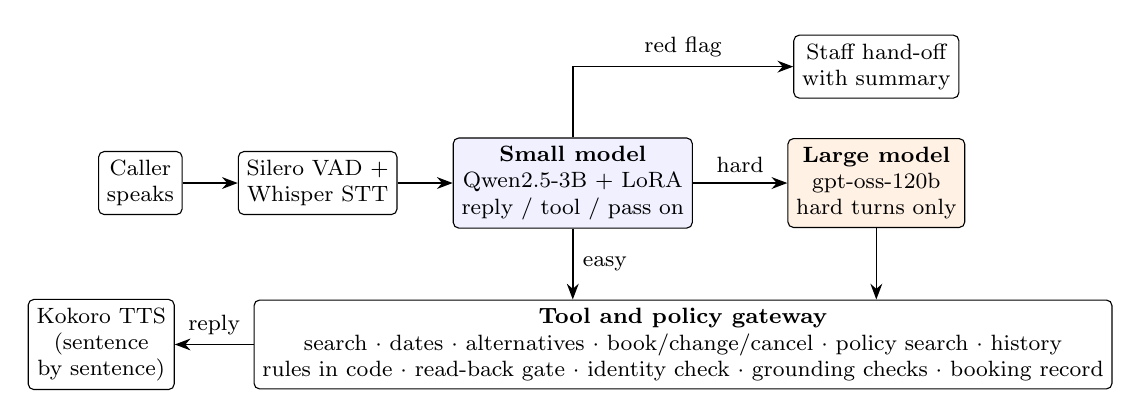
\begin{tikzpicture}[font=\footnotesize, node distance=6mm and 7mm,
  box/.style={draw, rounded corners=2pt, align=center, minimum height=8mm, inner sep=3pt, fill=white},
  arr/.style={-{Stealth[length=2mm]}, semithick}]
\node[box] (caller) {Caller\\speaks};
\node[box, right=of caller] (stt) {Silero VAD +\\Whisper STT};
\node[box, right=of stt, fill=blue!6] (small) {\textbf{Small model}\\Qwen2.5-3B + LoRA\\reply / tool / pass on};
\node[box, right=12mm of small, fill=orange!10] (large) {\textbf{Large model}\\gpt-oss-120b\\hard turns only};
\node[box, above=5mm of large] (staff) {Staff hand-off\\with summary};
\node[box, below=9mm of small, xshift=14mm] (gw) {\textbf{Tool and policy gateway}\\ search $\cdot$ dates $\cdot$ alternatives $\cdot$ book/change/cancel $\cdot$ policy search $\cdot$ history\\
rules in code $\cdot$ read-back gate $\cdot$ identity check $\cdot$ grounding checks $\cdot$ booking record};
\node[box, left=10mm of gw] (tts) {Kokoro TTS\\(sentence\\by sentence)};
\draw[arr] (caller) -- (stt);
\draw[arr] (stt) -- (small);
\draw[arr] (small) -- node[above]{hard} (large);
\draw[arr] (small.north) |- node[pos=0.75, above]{red flag} (staff.west);
\draw[arr] (small) -- node[right]{easy} (gw.north -| small);
\draw[arr] (large.south) -- (gw.north -| large);
\draw[arr] (gw) -- node[above]{reply} (tts);
\end{tikzpicture}
\caption{FastLane. Every caller turn goes to the tuned small model, which replies (optionally with a tool call),
passes the turn to the large model, or hands it to staff. Neither model writes to the booking system directly.}
\label{fig:arch}
\end{figure}

\paragraph{Practice world.} One SQLite database built from a fixed seed with a fixed ``now'' (Thursday 15 October
2026, so Dussehra and Diwali fall inside the booking window): 4 cinemas, 12 screens, 9 films and 1,440 shows with
seat maps (41,110 seats taken); 6 bus routes between Hyderabad and Bengaluru, Vijayawada and Chennai with 720 trips
(6,966 seats taken); 3 Tandoor Tales branches with 45 tables and 2,613 existing reservations; 200 callers with 510
past bookings (for returning callers) and 70 open bookings. Some shows, trips and slots are sold out on purpose for
the ``needs an alternative'' calls. Each test call starts from a snapshot of the same database.

\paragraph{Gateway and rules.} The gateway exposes eleven tools with validated arguments:
\cmd{search\_inventory}, \cmd{resolve\_date}, \cmd{find\_alternatives}, \cmd{create\_booking}, \cmd{modify\_booking},
\cmd{cancel\_booking}, \cmd{lookup\_booking}, \cmd{get\_caller\_history}, \cmd{search\_policy}, \cmd{send\_sms} and
\cmd{handoff\_to\_staff}. Rules are enforced in code, not in the prompt:
at most 10 movie tickets and changes up to 4\,h before the show; at most 6 bus seats, name/age/gender for every
passenger, refunds of 90/75/50/25\% by hours to departure; restaurant party limits (12/10/8 by branch) and a deposit
for large groups. A create, change or cancel first returns a read-back that must be spoken to the caller; the same
call succeeds only after the caller confirms it in the next turn. Changes need the phone number of the booking.
Four rules were added after observed failures (Section~\ref{sec:impl}): \emph{passenger source} (every bus
passenger's name and age must have been said by the caller or come from their history, and the passenger count must
cover the seats asked for), \emph{grounding} (the booked venue and time must have been said by the caller or offered
by the agent earlier in the call), \emph{heard count} (a ticket count or party size must be a number the caller said)
and \emph{origin heard} (a bus search from a city other than Hyderabad needs the caller to have named it). There is no payment tool; SMS is only logged.

\paragraph{Booking record and retrieval.} A typed per-domain record (film/route/branch, date, time, count,
passengers, name, read-back status) is shared by both models and the staff summary. Policy questions use a BM25~\cite{bm25}
index over 25 policy documents (fares, refund rules, FAQs, allergen-tagged menus, a
festival calendar, an old and a current version of the bus refund policy); a lookup starts on partial transcripts
and is reused if the final transcript matches (early lookup).

\paragraph{Routing.} The small model outputs one JSON object: \cmd{route} (self / llm / staff), the slots heard this
turn, an optional tool call and the words to say. A turn goes to the large model when the small model routes it there
or its escalation score (from token log-probabilities) exceeds a threshold, and in code on a tool error, no
availability, a changed earlier choice, an unconfident policy match, a repeated tool call, and (added after
failures) a policy answer with numbers or a ``no'' answer after a policy search, a refund or fee figure given with no
search, or a reply that claims a booking change the gateway did not make. It goes to staff on the small model's ``staff'' route or two failed tool calls in a row. The large model gets
the booking record, the last turns and the same tools, finishes the turn, and returns control. Read-back confirmations
and goodbyes are templates that need no model call.

\paragraph{Models and serving.} Large model: \cmd{openai/gpt-oss-120b}~\cite{gptoss} on Groq (free tier during development, paid
tier with no backup for the final runs), during development with \cmd{gemini-3.5-flash} as a backup when Groq would make a call wait more than 10\,s (capped at 20\,s, no retry);
every response records which model answered, and rate-limit waiting is logged separately (\cmd{throttle\_ms}) and
never counted as model time. Simulated caller: Qwen2.5-7B~\cite{qwen25}, local. Small models, tuned and untuned, run as 4-bit MLX~\cite{mlx}
models (1.6\,GB) on a 16\,GB Apple M4 behind an OpenAI-compatible server that returns log-probabilities, so both are
timed on the same stack.

% =====================================================================================================================
\subsection{Implementation and fixes}\label{sec:impl}

\paragraph{Code base.} FastLane is one Python package (about 10,600 lines in \cmd{src/fastlane}) with one command-line
tool, \cmd{fastlane}, and 218 unit tests (about 1,750 lines) that run in 18\,s without any model or network, using
scripted model clients. Every long job is resumable: an evaluation run skips calls already in its results file, the
speech round trip caches every clip, and training finishes from a saved adapter. The raw results of every run are
in \cmd{results/}.
Table~\ref{tab:modules} lists the parts.

\begin{table}[tbp]
\centering\small
\begin{tabularx}{\linewidth}{@{}l>{\raggedright\arraybackslash}p{0.27\linewidth}L@{}}
\toprule
Package & What it does & How (main choices) \\
\midrule
\cmd{world} & practice world & SQLite schema and a seeded generator (fixed ``now'', planned sold-out cases, 200 callers with history); seat maps for cinemas and sleeper/seater buses \\
\cmd{gateway} & the only way to the data & 11 tools with typed arguments (pydantic); rules, read-back gate, identity check and grounding checks in code; spoken-date resolver; fuzzy matching of names said over the phone; the shared booking record \\
\cmd{agent} & orchestrator & per-turn routing (small $\to$ large $\to$ staff), escalation triggers in code, templates for read-backs, confirmations and goodbyes, a timed trace of every turn \\
\cmd{models} & model clients & one OpenAI-compatible client for Groq, Gemini, Ollama and MLX (rate-limit headers, \cmd{throttle\_ms}, backup model); prompts; parser for the small model's JSON; escalation score from log-probabilities \\
\cmd{retrieval} & policy search & BM25 index over 25 policy documents; early lookup on partial transcripts; 67-question retrieval test \\
\cmd{training} & practice calls and fine-tuning & rule-based caller and agent produce training steps through the real gateway; speech noise (rules, later TTS$\to$STT round trip); Kaggle QLoRA notebook; local merge and 4-bit MLX conversion; offline step check \\
\cmd{eval} & experiments & 360 scripted test calls, simulated caller (Qwen2.5-7B), scorer (outcome, hand-off, answer), metrics (success with Wilson CI, p50/p95, router recall, unsafe writes), reports and plots \\
\cmd{speech} & voice demo & browser page and WebSocket server: Silero VAD, Whisper large-v3-turbo (MLX) with a domain word list, the same agent, Kokoro TTS sentence by sentence; WER tools for the STT comparison \\
\bottomrule
\end{tabularx}
\caption{Packages of the implementation.}
\label{tab:modules}
\end{table}

\paragraph{How changes were made.} Every fix below started from an observed failure (a crashed run, a failed test
call, a voice-demo call, or a wrong offline step), was written as a unit test first where possible, and was then
checked against the generated training data: after each gateway rule, all 650 practice calls were regenerated through
the new code to confirm that the rule never blocks a correct booking (every time: no training example changed), so
no retraining was needed for code fixes. Fixes to the agent were never applied in the middle of a comparison run; a
fixed system is reported as a separate run.

\paragraph{Everything fixed.} Table~\ref{tab:allfixes} lists every fix in order, with the problem that led to
it, how it works, and its effect. Rows 1--10 concern infrastructure and training, rows 11--37 the agent, the gateway,
the data and the evaluation.

{\small
\setlength{\tabcolsep}{4pt}
\begin{longtable}{@{}r>{\raggedright\arraybackslash}p{0.07\linewidth}>{\raggedright\arraybackslash}p{0.30\linewidth}>{\raggedright\arraybackslash}p{0.53\linewidth}@{}}
\caption{Every fix in the implementation: the problem that showed it, and what was changed.}\label{tab:allfixes}\\
\toprule
\# & Date & Problem (where it showed) & Fix: how it works, and effect \\
\midrule
\endfirsthead
\multicolumn{4}{@{}l}{\small\emph{Table~\ref{tab:allfixes} continued}}\\
\toprule
\# & Date & Problem (where it showed) & Fix: how it works, and effect \\
\midrule
\endhead
\bottomrule
\endfoot
\multicolumn{4}{@{}l}{\emph{Infrastructure, serving and training}}\\
1 & 20 Oct & Groq free tier: 8k tokens/min; waits would inflate latency & the client reads \cmd{retry-after} and remaining-token headers and waits before sending; waiting is stored as \cmd{throttle\_ms}, never as model time \\
2 & 21 Oct & pilot hit Groq's daily limit (10--15 min waits per turn) & \cmd{FallbackClient}: a call that would wait $>$10\,s goes to \cmd{gemini-3.5-flash}; every reply records which model answered; tool history is rewritten as text for Gemini, which needs its own \cmd{thought\_signature} \\
3 & 25 Oct & Kaggle run 1 crashed at step 1 (bfloat16 in the fp16 loss scaler) & trainable LoRA weights cast to float32, leftover bfloat16 base weights to float16; the notebook stops at the first failed step \\
4 & 25 Oct & adapter merge failed on Kaggle (\cmd{torchao} vs \cmd{peft}) & \cmd{torchao} uninstalled; a failed merge no longer fails the run; merging is done locally \\
5 & 25 Oct & Ollama cannot import a LoRA-tuned Qwen2 & small models served as 4-bit MLX models by \cmd{fastlane serve} (OpenAI-compatible, with log-probabilities); the untuned base is converted the same way, so both are timed on one stack \\
6 & 26 Oct & the first ``v2'' check gave exactly v1's output & a stale merged folder was re-quantised; the merge now always starts from scratch, and weight hashes are compared before a model is evaluated \\
7 & 26 Oct & one Gemini backup reply took 45.6\,s & backup capped at 20\,s with no retry; if it fails the call waits for Groq and the lost time counts as waiting \\
8 & 28 Oct & the Kaggle run meant for data v4 trained v3 again (old dataset attached) & the notebook asserts exactly one data folder, the expected example counts and the noise type before training; v5 was then trained correctly (7 Nov) \\
9 & 9 Nov & Groq unreachable for $\sim$40 min; 4 calls told the caller ``Sorry, I didn't quite get that'' & the backup is also used for 30\,s after a connection error or a 5xx reply (not only on rate limits); other errors still raise \\
10 & 10 Nov & Gemini's free tier allows 20 requests/day; the final runs need $\sim$1,500 & final runs on Groq's paid tier with the backup switched off, so every system sees only gpt-oss-120b \\
\midrule
\multicolumn{4}{@{}l}{\emph{Pilot v0 (untuned small model), 21 Oct}}\\
11 & 21 Oct & large-model turns crashed with HTTP 400 (\cmd{gender: "female"} vs schema \cmd{M/F/O}) & lenient schema plus normalisation in the gateway; provider-side argument rejections are fed back to the model, which retries \\
12 & 21 Oct & the large model asked for passengers three times & arguments passed to write tools now fill the booking record, so details survive a refused call and a switch between models \\
13 & 21 Oct & ``Friday 23rd October'' booked on Friday 16th & an explicit day of the month beats a weekday word \\
14 & 21 Oct & \cmd{"10:00"} searched as 10 PM & ``bare hour = PM'' applies only to spoken times; two-digit \cmd{HH:MM} is literal \\
15 & 21 Oct & ``\ldots 44, male, that's all'' ended the call & a goodbye must be a short turn with no numbers \\
16 & 21 Oct & correct policy answers scored wrong (narrow no-break space in ``4 hours'') & the scorer normalises Unicode spaces and dashes; stored calls rescored \\
17 & 21 Oct & the simulated caller hung up right after ``yes'' & caller prompt: hang up only after a reference, an answer or a transfer \\
\midrule
\multicolumn{4}{@{}l}{\emph{Training data and model versions}}\\
18 & 25 Oct & v1: every remaining offline error involved a date & the small model copies the caller's own words for a date; code resolves them (\cmd{resolve\_date}, also inside search and alternatives) and stores the ISO date in the record; wrong resolutions over all 360 spoken date forms: 69 $\to$ 0. Retrained as v2 \\
19 & 26 Oct & A2 (no date tools): the date the large model worked out was lost on the next turn & the small model carries that date as \cmd{YYYY-MM-DD} in its slots; only A2 steps changed (data v3, adapter v3) \\
20 & 26 Oct & voice demo: details given together in one sentence were dropped; ``Which cinema?'' in a bus call & data v4: openings with 0--5 details in random order, 35\% without a domain word \\
21 & 27 Oct & 14.9\% of rule-based noise copies lost a detail the target still had (``four tickets'' $\to$ ``for tickets'' with quantity 4) & data v5: noise copies from a real TTS$\to$phone-channel$\to$Whisper round trip, kept only if every key detail survives \\
\midrule
\multicolumn{4}{@{}l}{\emph{Pilot v3 and the voice demo, 26--27 Oct}}\\
22 & 26 Oct & invented passenger ``Caller (40)''; 1 of 3 seats booked & \emph{passenger-source rule}: every passenger's name and age must have been said in the call (digits or words) or come from the caller's history, and the passengers must cover the seats asked for; rerun 3/3 \\
23 & 26 Oct & refund table misread (90\% instead of 25\%) & a small-model policy answer with numbers goes to the large model with the same search result \\
24 & 26 Oct & voice demo: search with a cinema nobody named, the caller's 7 PM dropped & \emph{grounding rule}: the booked venue (cinema, bus destination and non-Hyderabad origin, branch) and time must have been said by the caller or offered by the agent; the agent's own read-backs do not count \\
25 & 26 Oct & voice server: every WebSocket got HTTP 403; SQLite used from another thread & annotation import fixed; one worker thread per call \\
26 & 27 Oct & hand-off announced but no tool called; markdown read aloud; the page hid ``call ended'' & a reply that says it \emph{is} transferring hands off in the same turn; every reply is converted to plain sentences; the page waits for the last audio, then shows the transfer notice \\
\midrule
\multicolumn{4}{@{}l}{\emph{Before the final runs, 6 Nov}}\\
27 & 6 Nov & ``Authenticates'' (misheard) booked as 4 tickets & \emph{heard-count rule}: a ticket count or party size must be a number the caller said (digits, words, Hindi numerals, ``just me'', ``one more'') or one the agent offered \\
28 & 6 Nov & A8: half the restaurant calls sent \cmd{quantity} instead of \cmd{party\_size} & the gateway reads \cmd{quantity} as \cmd{party\_size} for restaurants \\
29 & 6 Nov & B1 booked every movie twice: ungated tools still described a read-back & without the gate (B1, A3), write tools say ``the booking is made as soon as you call this; read back first, call once''; B1 and A3 rerun \\
30 & 6 Nov & the small model made the same policy search 4 times ($\approx$7\,s) & a repeated successful tool call in the same turn goes to the large model at once \\
31 & 6 Nov & router recall counted every relative date as a hard turn & second metric in which a date-only turn is not hard when the date tools exist; the original metric is kept \\
\midrule
\multicolumn{4}{@{}l}{\emph{v5 check, 9 Nov}}\\
32 & 9 Nov & ``Your refund will be 100\%'' with no policy search & a refund, fee, deposit, charge or percentage figure with no search this turn goes to the large model \\
33 & 9 Nov & ``4-hour'' scored as not matching ``4 hours'' & the scorer reads ``N-hour'' as ``N hours''; no success value changed on rescoring \\
\midrule
\multicolumn{4}{@{}l}{\emph{After the final runs, 10 Nov (FastLane rerun as a separate run)}}\\
34 & 10 Nov & caller said only ``to Hyderabad''; the small model searched \emph{from Bengaluru} and the call ended on the wrong bus (2 calls) & \emph{origin-heard check at search time}: a bus search or alternatives request from a city other than Hyderabad needs the caller to have said that city (aliases count; the agent's own words do not) or the city to come from the caller's history or a booking verified in the call; checked before the result fills the record, so a guessed city never reaches it \\
35 & 10 Nov & the gateway refused a cancellation (no clear yes), and the small model said ``Your booking was cancelled'' & \emph{completion-claim check}: a reply saying a change was made (``was cancelled'', ``has been booked'', ``I've changed it'') while the last change tried in the call did not go through goes to the large model; a large-model reply doing the same gets one correction and retries \\
36 & 10 Nov & search found ``Mall parking (Rs 60 for 4 hours)''; the small model said ``No parking facility'' & a ``no'' or ``not'' answer from the small model after a policy search goes to the large model with the same result \\
37 & 10 Nov & after-fix run: ``Can you please confirm my name and phone number?'' counted as a yes to a cancellation read-back (it contains ``confirm'') & a question is \emph{unclear}, not a yes, unless it starts with a yes-word (``Yes, can you also send the SMS?''); the agent asks again. Among all answers to read-backs in the final runs this changes only that call \\
\end{longtable}
}

\noindent On the 120 final-run transcripts, rows 35 and 36 would have fired on exactly 3 small-model turns: the two
errors they target and ``No, the dal makhani is not nut-free'', which turned out to be a third error (the menu says it
contains no nuts). The effect of rows 34--37 is reported in Section~\ref{sec:afterfix}.

\paragraph{A training-data defect found through row 34.} Checking the origin rule against the practice-call generator
showed why the model guesses a city: in four sold-out bus calls to Hyderabad the generated caller says only
``6 seats to Hyderabad'', and the rule-based agent that writes the training targets searches from the trip's real
origin without asking. These are 6 of the 225 bus-search steps in data v3 (and v5). With the new rule the generator
drops exactly these 4 calls (641 of 650 kept, no other example changes). There was no time to retrain before the
deadline, so the rule in the gateway is the fix; a regenerated data set would remove the pattern at its source.


% =====================================================================================================================
\subsection{Training data and fine-tuning}\label{sec:training}

\paragraph{Generator.} Instead of an LLM teacher, both sides of each practice call are code: a rule-based caller that
follows a plan (domain, kind of call, which details it gives and when) and an oracle agent that knows the ideal next
step. The calls run through the \emph{real} orchestrator and gateway, and every small-model call is stored as (exact
input, ideal JSON output), so training inputs match inference byte for byte and are free to produce. Only calls that
end in the planned final state are kept (645 of 650). Routing targets follow the proposal: changed choices, ``my
usual'' and refused details go to the large model; red flags, deposit waivers and over-limit groups go to staff;
no-availability and tool errors escalate in code. Prompts are mixed (FastLane 60\%, A2 15\%, A4 10\%, A6 5\%, A7 10\%)
so one adapter works with every variant's tool list and context. Escalation steps (about 5\% of steps) are repeated
3$\times$ in training only. About 30\% of training steps get a speech-noise copy (Section~\ref{sec:noise}). The
tuned model gets a 643-token system prompt instead of 1,062 (less prefill time). Data is split by call, 90/10.

\paragraph{Do people agree with the routing labels?} Two team members labelled 300 first-step turns (the last three
lines of a practice call, stratified by the rule label: 175 self, 75 llm, 50 staff) as self, llm or staff, each on
their own and without the rule label (Table~\ref{tab:kappa}). They agree on 187 turns (62\%), Cohen's
$\kappa = 0.17$~\cite{cohen}; against the rule labels $\kappa = 0.65$ (A) and $0.42$ (B). The disagreement is not spread out. On
plain bookings, dates and sold-out turns both annotators agree with each other on 127 of 128 turns. It sits in turns
whose label is a design decision the annotators were not given: B sent every policy question, cancel request and
deposit waiver and 7 of 9 change-of-booking requests to the large model and kept changes of mind with the small
model, while A kept
``my usual'' and refused-passenger-details turns with the small model. Neither sent over-limit group requests to
staff, as the design does. Seven date turns are llm only because they come from the A2 prompt (no date tool), which
the sheet does not show. Our short instructions to the annotators also listed policy questions under llm, which
the design does not do (the small model answers them from the retrieved text). So the rule labels are one
consistent reading of the routing policy; without a written guideline people read it differently, and $\kappa$
here mostly measures the missing guideline. There was no time for a second round with written guidelines.

\begin{table}[tbp]
\centering\small
\begin{tabularx}{\linewidth}{@{}L r r r r@{}}
\toprule
Kind of turn & Turns & A = B & A = rule & B = rule \\
\midrule
Plain booking, dates, sold out & 128 & 127 & 121 & 120 \\
Change of mind & 59 & 25 & 59 & 25 \\
``My usual'' / same bus as last time & 26 & 3 & 3 & 26 \\
Red flag (complaint, refund, lost item, out of scope) & 26 & 20 & 26 & 20 \\
Refuses passenger details & 14 & 5 & 5 & 14 \\
Group over the limit (rule: staff) & 14 & 5 & 0 & 0 \\
Deposit waiver (rule: staff) & 10 & 0 & 10 & 0 \\
Cancel, modify, policy question & 23 & 2 & 23 & 2 \\
\midrule
All & 300 & 187 & 247 & 207 \\
Cohen's $\kappa$ & & 0.17 & 0.65 & 0.42 \\
\bottomrule
\end{tabularx}
\caption{Agreement on routing labels (self / llm / staff) between two annotators and the rule labels used for
training, by kind of practice call.}
\label{tab:kappa}
\end{table}

\paragraph{Training.} QLoRA~\cite{qlora,lora} on a Kaggle T4: 4-bit base, rank 16, $\alpha$=32, dropout 0.05, all seven projection
matrices, learning rate $2\cdot10^{-4}$ with cosine decay and 3\% warm-up, effective batch 16, 2 epochs, sequence
length 2,048, loss on the target JSON only. Adapters are merged and converted to 4-bit MLX locally.
Table~\ref{tab:data} lists the data versions and Table~\ref{tab:runs} the training runs; Figure~\ref{fig:loss} shows
that validation loss flattens from about epoch 1.7, so two epochs are enough.

\begin{table}[tbp]
\centering\small
\begin{tabularx}{\linewidth}{@{}l r r L@{}}
\toprule
Data & Train & Val & What changed and why \\
\midrule
v1 & 3,722 & 273 & first version; 3,095 self / 411 llm / 216 staff in train; rule-based noise copies \\
v2 & 3,671 & 267 & spoken dates go in a slot and are resolved in code (v1 errors were all dates); A2 escalates every spoken date; ``Friday the 23rd'' fixed; 516 llm targets \\
v3 & 3,671 & 267 & A2 only: after the large model says a date back, the small model stores it as ISO (v2 labels were unlearnable) \\
v4 & 3,337 & 245 & callers give 0--5 details in any order, 35\% without the domain word (voice demo dropped details) \\
v5 & 3,153 & 245 & v4 calls; noise copies from a TTS$\rightarrow$STT round trip with a key-detail filter instead of rules \\
\bottomrule
\end{tabularx}
\caption{Training data versions (all-domains set; steps). Every version keeps 645 of 650 generated calls.}
\label{tab:data}
\end{table}

\begin{table}[tbp]
\centering\small
\begin{tabularx}{\linewidth}{@{}l l r r r L@{}}
\toprule
Run & Data & Opt.\ steps & Time & Val loss & Notes \\
\midrule
v1 (run 1) & v1 & -- & -- & -- & failed at step 1: bfloat16 LoRA weights on a T4 (fix: cast trainable weights to float32) \\
v1 (run 2) & v1 & 466 & 3\,h 17\,m & 0.0128 & token acc.\ 99.31\%; merge on Kaggle failed (torchao), merged locally \\
v2 all-domains & v2 & 460 & 3\,h 16\,m & 0.0118 & token acc.\ 99.30\% \\
v2 movies+buses (A8) & v2 & 332 & 2\,h 20\,m & 0.0152 & 2,644 train / 165 val; token acc.\ 99.27\% \\
v3 all-domains & v3 & 460 & 3\,h 22\,m & 0.0105 & token acc.\ 99.39\%; current model \\
v3 repeat & v3 & 460 & 3\,h 29\,m & 0.0113 & run meant for v4 used the old dataset version; shows run-to-run variation \\
\bottomrule
\end{tabularx}
\caption{Kaggle training runs (one T4, QLoRA). Validation sets differ between data versions, so losses across rows
are not strictly comparable.}
\label{tab:runs}
\end{table}

\begin{figure}[tbp]
\centering
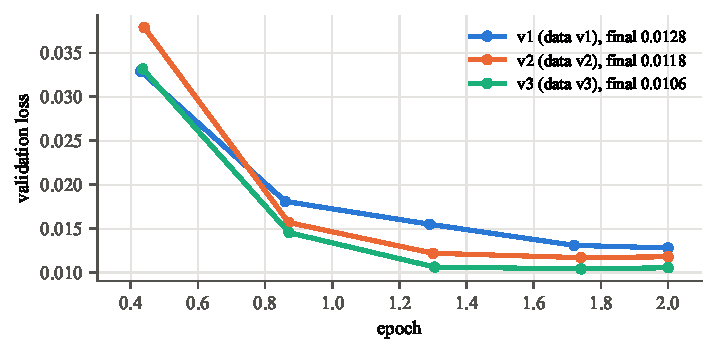
\includegraphics[width=0.72\linewidth]{figures/loss_curves.pdf}
\caption{Validation loss of the all-domains adapters by epoch (each on its own data version's validation set).}
\label{fig:loss}
\end{figure}

% =====================================================================================================================
\section{Experiment Runs}\label{sec:eval}

\paragraph{Baselines and ablations.} One configuration object defines all 12 systems of the proposal
(Table~\ref{tab:systems}). Baselines (B1--B3) are other ways someone could build the same agent; ablations (A1--A8)
are FastLane with exactly one part removed or changed, so each differs from FastLane in one flag. All 12 run end to
end.

\paragraph{Final runs.} The final runs (10 November) use the code of 9 November (rows 1--33 of
Table~\ref{tab:allfixes}), adapter v3 and \cmd{openai/gpt-oss-120b} on Groq's paid tier with the backup model
switched off, so every system sees the same large model. FastLane and B1 run on a stratified sample of 120 test calls
(40 per domain, 15 per category); B2, B3 and A1--A7 run on 48 of these calls (16 per domain, 6 per category). The
samples are nested and contain the 24 calls used during development, so 96 of the 120 calls were never looked at
before the final run. A8 is run as a matched pair: the all-domains and the movies+buses adapters, both trained on data
v5, on the same 40 restaurant calls. Each system is compared with FastLane on the same calls with an exact McNemar
test~\cite{mcnemar}. The offline ablations on held-out steps cover A1 (untuned vs.\ tuned) and A8 (new domain), and a data ablation
compares rule-based with round-trip speech noise (v3 vs.\ v5, Section~\ref{sec:noise}).

\begin{table}[tbp]
\centering\small
\begin{tabularx}{\linewidth}{@{}lL@{}}
\toprule
System & How it differs from FastLane \\
\midrule
FastLane & tuned small model on every turn; hard turns to the large model or staff; code tools, gateway, record, early lookup, caller history \\
B1 & large model only, booking rules in the prompt (how most voice agents work) \\
B2 & untuned small model only; large model never used \\
B3 & the large model is asked before every turn whether it is easy or hard \\
A1--A8 & no fine-tuning (A1); no date/alternative tools (A2); rules only in the prompt, no read-back (A3); no booking record (A4); no step-by-step reasoning for the large model (A5); no early lookup (A6); no caller history (A7); small model trained on movies+buses only, tested on restaurants (A8) \\
\bottomrule
\end{tabularx}
\caption{The 12 systems of the proposal, all implemented as presets of one configuration.}
\label{tab:systems}
\end{table}



\paragraph{All runs.} Table~\ref{tab:allruns} lists every experiment run in this report, in the order they were made.
The test calls are described in Section~\ref{sec:data}.

\begin{table}[tbp]
\centering\small
\begin{tabularx}{\linewidth}{@{}>{\raggedright\arraybackslash}p{3.0cm}LL>{\raggedright\arraybackslash}p{2.1cm}@{}}
\toprule
Run & Systems and data & Purpose & Results \\
\midrule
Retrieval evaluation & BM25 on 67 policy questions & choose the retrieval thresholds & Section~\ref{sec:retrieval} \\
Recogniser comparison & 3 recognisers ($\pm$ domain word list) on 300 Svarah clips and 142 booking lines & choose the recogniser & Table~\ref{tab:stt} \\
Offline step checks & untuned base and the tuned adapters on 267 held-out steps & model development; offline A1 and A8 & Table~\ref{tab:offline}, Section~\ref{sec:rq3off} \\
Pilot (21 Oct) & FastLane with the untuned and the tuned small model & first end-to-end check & Section~\ref{sec:pilot} \\
Development runs & all 12 systems on 24 calls (mid-submission); B1, B3, A3 again on 6--7 Nov & find failures and fix them & Section~\ref{sec:fixes}, Table~\ref{tab:allfixes} \\
Data v5 check (7--9 Nov) & adapters v3 and v5, offline and on 24 calls & choose the adapter; rule-based vs.\ round-trip noise & Section~\ref{sec:noise} \\
Final runs (10 Nov) & FastLane, B1 on 120 calls; B2, B3, A1--A7 on 48; A8 pair on 40 restaurant calls & main comparison & Table~\ref{tab:baselines}, Section~\ref{sec:ablations} \\
After-fix run (10 Nov) & FastLane with the fixed code on the same 120 calls & effect of four fixes; run-to-run variation & Section~\ref{sec:afterfix} \\
Label agreement (11 Nov) & 300 turns, 2 annotators & check the routing labels & Table~\ref{tab:kappa} \\
\bottomrule
\end{tabularx}
\caption{All experiment runs. The final runs use one seed and gpt-oss-120b on Groq's paid tier for every system.}
\label{tab:allruns}
\end{table}

\paragraph{Metrics.} Success = the set of bookings created or changed matches one acceptable gold outcome exactly
(plus hand-off and policy-answer expectations), with Wilson 95\% intervals~\cite{wilson}. Speed = model time per turn (p50/p95),
excluding rate-limit waiting. Also: share of turns sent to the large model, large-model calls and tokens per call,
router precision/recall on labelled hard turns, invalid tool calls, success on calls with injected errors, unsafe,
unconfirmed and rule-violating writes, missed hand-offs, and early-lookup statistics. Systems are compared on the
same calls with an exact McNemar test on per-call success.

\paragraph{Offline step check.} For model development we replay held-out validation steps (the exact small-model
input of a generated call) and compare the output with the target JSON: valid JSON, route accuracy, escalation
precision/recall, right tool and exact tool arguments (the arguments that decide the action; dates count as equal when
they name the same day). This needs no large model or simulated caller, so it is cheap and deterministic.

% =====================================================================================================================
% =====================================================================================================================
\section{Ablations}\label{sec:ablations}

Each ablation is FastLane with exactly one part removed or changed (Table~\ref{tab:systems}), so its difference from
FastLane on the same calls measures what that part contributes. In the final runs A1--A7 ran on the same 48 calls as
FastLane, and A8 ran as a matched pair on 40 restaurant calls (Section~\ref{sec:eval}). Table~\ref{tab:ablations}
summarises them; Table~\ref{tab:baselines} and Figure~\ref{fig:systems} (Section~\ref{sec:baselines}) give every
metric next to the baselines. Three ablations were also run offline: A1 on held-out steps (Table~\ref{tab:offline}),
A8 on held-out restaurant steps (Section~\ref{sec:rq3off}), and a data ablation of rule-based against round-trip
speech noise (Section~\ref{sec:noise}).

\begin{table}[tbp]
\centering\small
\setlength{\tabcolsep}{4pt}
\begin{tabular}{@{}llllrrr@{}}
\toprule
System & Part removed or changed & Tests & Success & $p$ & \hcell{Large calls\\per call} & \hcell{Unconfirmed-\\change calls} \\
\midrule
FastLane & -- & -- & 46/48 & -- & 1.67 & 0 \\
A1 & fine-tuning of the small model & RQ1 & 21/48 & $<$0.001 & 1.88 & 0 \\
A2 & date and alternative tools & H4 & 41/48 & 0.13 & 3.35 & 0 \\
A3 & rules and read-back in code & H5 & 35/48 & 0.001 & 2.21 & 31 \\
A4 & booking record & RQ2 & 42/48 & 0.22 & 2.77 & 0 \\
A5 & reasoning on hard turns & -- & 44/48 & 0.63 & 1.71 & 0 \\
A6 & early lookup & H7 & 43/48 & 0.25 & 1.69 & 0 \\
A7 & caller history & -- & 45/48 & 1.00 & 2.33 & 0 \\
\midrule
FastLane (v5)$^\dagger$ & -- & -- & 37/40 & -- & 0.90 & 0 \\
A8$^\dagger$ & restaurants in the training data & H6, RQ3 & 37/40 & 1.00 & 1.82 & 0 \\
\bottomrule
\end{tabular}
\caption{Ablations in the final runs, each against FastLane on the same calls ($p$: exact McNemar test). Unconfirmed-change
calls: calls with a booking change the caller never confirmed. $^\dagger$Restaurant calls only, both adapters trained
on data v5.}
\label{tab:ablations}
\end{table}

\paragraph{A1: no fine-tuning (RQ1).} With the untuned Qwen2.5-3B in place of the tuned one, and the large model
available, FastLane succeeds in only 21 of 48 calls ($p<10^{-7}$): 17\% of its tool calls are invalid, 18 calls reach
the turn limit, and no call with an injected tool error succeeds. The untuned model rarely passes a turn on by itself
(12.8\% of turns go to the large model, about half of them only after a failed tool call), so it keeps turns it cannot
do. Alone (B2, Section~\ref{sec:baselines}) it succeeds in 14 of 48. This is the one conclusion that changed since
development: the earlier A1 result (79.2\%) came from the first pilot (21 October), whose older code sent 60.7\% of
turns to the large model; it is not comparable with the final code. Offline the picture is the same: fine-tuning
lifts route accuracy from 89.1\% to 99.3\% and exact tool arguments from 26.8\% to 99.0\% (Table~\ref{tab:offline}).
Fine-tuning is what makes the small model usable.

\paragraph{A2: no date and alternative tools (H4).} Without \cmd{resolve\_date} and \cmd{find\_alternatives}, the
small model passes dates and sold-out shows on: the share of turns sent to the large model doubles (21.0\%
$\rightarrow$ 41.8\%), large-model calls per call double (1.67 $\rightarrow$ 3.35), large-model tokens per call rise
from 3.9k to 6.7k, and median model time per turn rises from 1.61\,s to 2.61\,s. Success falls from 46 to 41 of 48
($p=0.13$), mostly in changes of mind (3/6), dates and sold-out calls (5/6 each).

\paragraph{A3: rules only in the prompt, no read-back (H5).} With the same models but no gateway rules and no
read-back gate, \textbf{31 of 48 calls (65\%) made a booking change that the caller never confirmed} (40 of its 50
writes), and 9 writes in 9 calls broke a booking rule; only 1 of 6 rule-breaking requests ended correctly (FastLane
6/6). Success falls to 35 of 48 ($p=0.001$), and 20 of the 35 successful calls contained an unconfirmed change, so
task success alone understates the risk. The 24-call runs during development showed the same (13 of 24 calls).

\paragraph{A4--A7: the other components.} None of these changes success significantly on 48 calls; their effect
shows in large-model use. Without the booking record (A4, 42/48) the models must recover details from the chat, so
the large model gets more turns (30.2\% vs.\ 21.0\%; 2.77 calls per call); movie calls suffer most (12/16). Without
step-by-step reasoning on hard turns (A5, 44/48) the large model writes less than half the output tokens (169 vs.\
374 per call) with no loss we can measure. Without caller history (A7, 45/48) the large model is called more often
(2.33 calls per call), and one returning caller fails. Without early lookup (A6, 43/48) nothing changes measurably
(H7, Section~\ref{sec:status}).

\paragraph{A8: a small model never trained on restaurants (H6).} In the matched pair (both adapters trained on data
v5, the same 40 restaurant calls), the movies+buses adapter succeeds in 37 of 40 calls, exactly as many as the
all-domains adapter (one call differs each way). It has a slightly higher invalid tool-call rate (2.6\% vs.\ 1.7\%)
and makes twice as many large-model calls (1.82 vs.\ 0.90 per call). FastLane with
adapter v3 succeeds in 36 of the same 40 calls. The gap seen during development (6/8 vs.\ 7/8) came from the older v2
adapter and the \cmd{quantity}/\cmd{party\_size} field, which the gateway now accepts; with the same data version,
leaving restaurants out of training costs no success, only more large-model calls.

% =====================================================================================================================
\section{Evaluations}\label{sec:results}

This section evaluates each part and the whole system: retrieval, the small model offline, the pilot, the fixes,
the final comparison with the baselines and its failure analysis, the after-fix run, and the speech layer.

\subsection{Retrieval}\label{sec:retrieval}
On a 67-question policy QA set, BM25 retrieval reaches Recall@3 0.967, top-1 0.817, answer-in-context 0.883, covered
when answerable 0.933, current-policy choice 1.00 (old vs.\ new refund policy) and ``not covered'' detection 0.714
(only 7 such questions). The thresholds were tuned on the same set, so these numbers are optimistic.

\subsection{Offline step accuracy}\label{sec:offline}
Table~\ref{tab:offline} compares the untuned base with the tuned versions on the same 267 held-out steps and the same
4-bit MLX stack. Fine-tuning is what makes the small model usable: the untuned model routes 89.1\% of steps correctly
but escalates with 46\% precision and fills tool arguments exactly only 26.8\% of the time. v1 already routed 96.6\%
correctly; every one of its remaining errors involved dates (a date said early in the call had scrolled out of the
6-line context and was never stored, A2 date turns were not escalated, and \cmd{resolve\_date} read ``Friday the
23rd'' as the coming Friday: 69 of 360 spoken forms wrong). Data v2 fixed these in the data and the tools, raising
escalation recall from 65.4\% to 92.3\% and arguments from 90.5\% to 92.5\% (98.4\% in the FastLane configuration).
v3 removed a label bug in A2 (Section~\ref{sec:lessons}): on its own validation set, steps with any error fell from
15 (v2) to 6, and the date the large model says back is carried into the record in 7 of 10 A2 calls (v2: 0 of 10).

\begin{table}[tbp]
\centering\small
\begin{tabular}{@{}lrrrr@{\hspace{2em}}rr@{}}
\toprule
& \multicolumn{4}{c}{267 steps of data v2} & \multicolumn{2}{c}{267 steps of data v3} \\
\cmidrule(r{2em}){2-5}\cmidrule{6-7}
Metric & Untuned & v1 & v2 & & v2 & v3 \\
\midrule
Route accuracy & 89.1 & 96.6 & \textbf{98.9} & & 99.3 & 99.3 \\
Escalation precision & 46.2 & 100 & 96.0 & & 100 & 100 \\
Escalation recall & 23.1 & 65.4 & \textbf{92.3} & & 92.3 & 92.3 \\
Right tool & 49.8 & 96.7 & 96.7 & & 95.9 & \textbf{98.8} \\
Exact tool arguments & 26.8 & 90.5 & \textbf{92.5} & & 97.2 & \textbf{99.0} \\
p50 / p95 latency (s) & 2.20 / 7.55 & 2.22 / 4.83 & 2.22 / 4.51 & & 2.32 / 4.88 & 1.96 / 4.24 \\
\bottomrule
\end{tabular}
\caption{Offline step accuracy (\%) of the small model, same steps and serving stack within each block.}
\label{tab:offline}
\end{table}

\paragraph{Error analysis of v3.} The 6 remaining errors: two changes that call \cmd{modify\_booking} without
searching first, one \cmd{quantity} instead of \cmd{party\_size} in a restaurant change, one extra policy search, one
complaint handed to staff by calling the tool instead of routing (same outcome) and one missed A2 escalation.

\subsection{New domain (RQ3, offline)}\label{sec:rq3off}
The movies+buses adapter (A8) has never seen a restaurant call. On the 54 restaurant steps of data v2 it routes 98.1\%
correctly (all-domains v2: 100\%; untuned: 87.0\%), with escalation recall 88.9\% (100\%; 33.3\%) and the right tool
88.9\% of the time (95.6\%; 46.7\%). Argument filling does \emph{not} transfer: 47.6\% exact (100\%; 50.0\%), and all
11 errors are the same one, \cmd{quantity} (the movie/bus field) where restaurants need \cmd{party\_size}. The gateway
rejects such calls, so in a live call this costs an extra step or a hand-off. Routing transfers; the schema does not.

\subsection{Pilot: untuned vs.\ tuned small model}\label{sec:pilot}
Table~\ref{tab:pilot} compares two 24-call pilots (one call per domain $\times$ category
cell, same calls, same caller simulator and large model); only the small model changed. The tuned model keeps easy
turns: the share of turns sent to the large model falls from 60.7\% to 13.5\%, large-model tokens per call fall
5$\times$, the free-tier rate limit is never hit (110\,s of waiting per call $\rightarrow$ 0), and median model time
per turn falls by 42\%. Success rises from 79.2\% to 87.5\% (policy 0/3 $\rightarrow$ 2/3, sold out and change of mind
2/3 $\rightarrow$ 3/3). Two numbers got worse. \emph{p95} rose because the slowest turns are now booking turns where the
small model takes two steps in a row (search, then read-back: about 3\,s + 5\,s on MLX), plus one 45.6\,s Gemini
reply. \emph{Router recall} fell because the test labels mark every relative date as hard, while FastLane handles
dates on the small model with code tools by design; 5 of the 13 ``missed'' hard turns are such date turns, and those
calls succeeded. The intervals overlap (24 calls, one seed): this is a pilot, not the final comparison.

\begin{table}[tbp]
\centering\small
\begin{tabular}{@{}lrr@{}}
\toprule
24 calls & Pilot v0 (untuned) & Pilot v3 (tuned) \\
\midrule
Task success [95\% CI] & 79.2\% [59.5--90.8] & \textbf{87.5\%} [69.0--95.7] \\
Turns sent to the large model & 60.7\% & \textbf{13.5\%} \\
Large-model calls / tokens per call (in / out) & 6.12 / 12,013 / 1,051 & \textbf{1.04} / \textbf{2,316} / \textbf{200} \\
Rate-limit wait per call & 110.3\,s & \textbf{0\,s} \\
Model time per turn p50 / p95 & 2.88\,s / \textbf{6.89\,s} & \textbf{1.66\,s} / 8.06\,s \\
Router precision / hard-turn recall & 25.3\% / \textbf{90.5\%} & \textbf{76.5\%} / 56.5\% \\
Invalid tool calls & 7.6\% & \textbf{0.9\%} \\
Success with injected tool errors & 100\% & 100\% \\
Unsafe / unconfirmed / rule-breaking writes & 0 / 0 / 0 & 0 / 0 / 0 \\
Missed hand-offs & 0/3 & 0/3 \\
Success by domain (buses / movies / restaurants) & 6/8, 7/8, 6/8 & 5/8, 8/8, 8/8 \\
\bottomrule
\end{tabular}
\caption{24-call pilots with FastLane; only the small model differs (untuned Qwen2.5-3B vs.\ adapter v3).}
\label{tab:pilot}
\end{table}

\subsection{Failures and the fixes they led to}\label{sec:fixes}
All three failed calls of pilot v3 were buses, and all were the small model acting alone where it should not
(Table~\ref{tab:fixes}). No gateway rule was broken, but two calls showed that passenger details were not checked
against what the caller had actually said. The voice demo later showed a related gap (a search with a cinema nobody
named and without the time the caller gave), which led to the grounding rule. Both rules were checked against all 650
generated practice calls: the same 645 calls are kept and \emph{no} training example changes, so the rules never
block a correct booking in our data. After the fixes, the 3 failed calls were rerun and all 3 succeed.

\begin{table}[tbp]
\centering\small
\begin{tabularx}{\linewidth}{@{}lLL@{}}
\toprule
Call & What went wrong & Fix and outcome on rerun \\
\midrule
bus-dates-161 & asked ``Which cinema?'' in a bus call, then booked invented passengers (``Caller (40)'') & passenger-source rule: the booking is refused, the large model asks for both passengers; booked correctly \\
bus-rule\_break-236 & caller asked for 3 seats but gave 1 passenger; model booked 1 seat with an invented age & passenger-count check: two attempts refused, call handed to staff (an accepted outcome) \\
bus-policy-201 & small model misread the refund table (90\% instead of 25\% for 10\,h before departure) & policy answers with numbers go to the large model: answered 25\% \\
mov-sold\_out-056 & one Gemini backup reply took 45.6\,s & backup capped at 20\,s, no retry, lost time counted as waiting \\
\bottomrule
\end{tabularx}
\caption{Pilot v3 failures, the code fixes (no retraining) and the rerun.}
\label{tab:fixes}
\end{table}

\subsection{Final comparison}\label{sec:baselines}
Table~\ref{tab:baselines} gives every system on its own calls next to FastLane on the same calls, and
Figure~\ref{fig:systems} puts all systems on the same 48 calls. During development the same systems ran on 24 calls
(mid-submission, and B1, B3 and A3 again on 6--7 November); the final runs confirm every conclusion of those runs
except the one about A1 (Section~\ref{sec:ablations}). The ablation rows of the table are discussed in
Section~\ref{sec:ablations}.

\begin{table}[tbp]
\centering\footnotesize
\setlength{\tabcolsep}{3.2pt}
\resizebox{\linewidth}{!}{%
\begin{tabular}{@{}lrrrrrrrrr@{}}
\toprule
System & Calls & Success [95\% CI] & \hcell{FastLane,\\same calls} & \hcell{$p$\\(McNemar)} & \hcell{Large-model\\turns} & \hcell{Large calls\\per call} & \hcell{p50 / p95\\(s)} & \hcell{Invalid\\tool calls} & \hcell{Unconfirmed-\\change calls} \\
\midrule
\textbf{FastLane} & 120 & \textbf{90.0\%} [83--94] & -- & -- & 20.9\% & 1.76 & 1.67 / 6.81 & 1.2\% & \textbf{0} \\
B1 large only & 120 & 81.7\% [74--88] & 108 & 0.087 & 100\% & 8.02 & \textbf{1.04} / \textbf{3.01} & 0.6\% & 44 \\
\midrule
\textbf{FastLane} & 48 & \textbf{95.8\%} [86--99] & -- & -- & 21.0\% & 1.67 & 1.61 / 6.70 & 1.3\% & \textbf{0} \\
B1 large only & 48 & 81.2\% [68--90] & 46 & 0.065 & 100\% & 8.42 & \textbf{1.01} / \textbf{3.12} & 1.6\% & 19 \\
B2 untuned small & 48 & 29.2\% [18--43] & 46 & $<$0.001 & 0\% & 0 & 1.65 / 16.08 & 27.6\% & 0 \\
B3 large as router & 48 & 91.7\% [80--97] & 46 & 0.50 & 76.0\% & 6.94 & 1.66 / 7.66 & 0.8\% & 0 \\
A1 no fine-tuning & 48 & 43.8\% [31--58] & 46 & $<$0.001 & 12.8\% & 1.88 & 1.53 / 5.52 & 17.0\% & 0 \\
A2 no date tools & 48 & 85.4\% [73--93] & 46 & 0.13 & 41.8\% & 3.35 & 2.61 / 8.65 & 3.1\% & 0 \\
A3 rules in prompt & 48 & 72.9\% [59--83] & 46 & 0.001 & 27.8\% & 2.21 & 2.28 / 7.50 & 6.4\% & 31 \\
A4 no booking record & 48 & 87.5\% [75--94] & 46 & 0.22 & 30.2\% & 2.77 & 1.76 / 6.55 & 1.8\% & 0 \\
A5 no reasoning & 48 & 91.7\% [80--97] & 46 & 0.63 & 21.1\% & 1.71 & 1.70 / 7.18 & 1.3\% & 0 \\
A6 no early lookup & 48 & 89.6\% [78--96] & 46 & 0.25 & 19.7\% & 1.69 & 1.68 / 7.11 & 1.2\% & 0 \\
A7 no caller history & 48 & 93.8\% [83--98] & 46 & 1.00 & 24.7\% & 2.33 & 1.81 / 7.03 & 3.3\% & 0 \\
\midrule
FastLane, adapter v5 & 40$^\dagger$ & 92.5\% [80--97] & -- & -- & 15.1\% & 0.90 & 1.60 / 7.39 & 1.7\% & 0 \\
A8 movies+buses v5 & 40$^\dagger$ & 92.5\% [80--97] & 37 & 1.00 & 24.2\% & 1.82 & 1.76 / 7.54 & 2.6\% & 0 \\
\bottomrule
\end{tabular}}
\caption{Final runs (one seed; gpt-oss-120b on Groq's paid tier for every system). ``FastLane, same calls'' is the
number of the system's calls that FastLane completed successfully; $p$ is the exact McNemar test on the same calls.
No rate-limit waiting occurred. Unconfirmed-change calls: calls with a booking change
the caller never confirmed. $^\dagger$Restaurant calls only; both adapters trained on data v5 (matched pair for A8).}
\label{tab:baselines}
\end{table}

\begin{figure}[tbp]
\centering
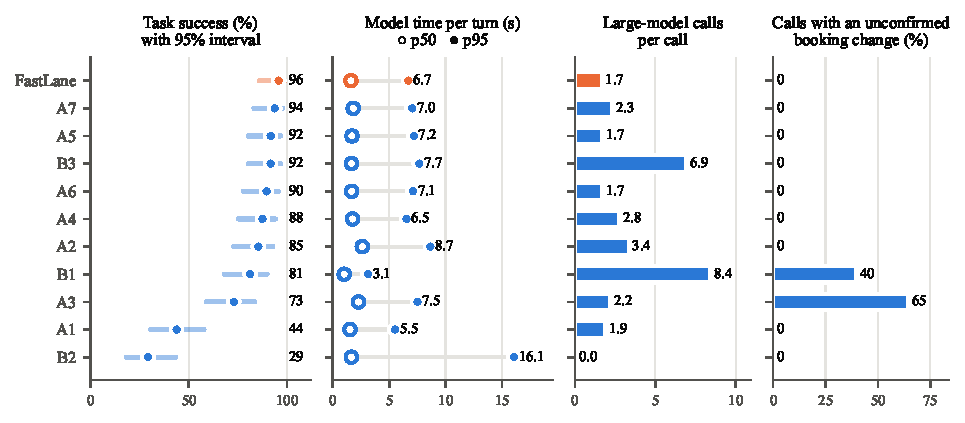
\includegraphics[width=\linewidth]{figures/systems_final.pdf}
\caption{All systems on the same 48 calls, sorted by task success: success with its 95\% interval, model time per
turn (p50 hollow, p95 filled), large-model calls per call, and the share of calls with a booking change the caller
never confirmed. FastLane in orange.}
\label{fig:systems}
\end{figure}

\paragraph{FastLane vs.\ the large model alone (B1; H1, H2).} On 120 calls FastLane succeeds in 108 (90.0\%) and B1
in 98 (81.7\%). Paired on the same calls, 19 calls succeed only with FastLane and 9 only with B1 ($p=0.087$), so the
gap points one way but is not significant; on the 96 calls never used during development it is 85 vs.\ 79. B1 loses
most on sold-out calls (8/15 vs.\ 14/15) and changes of mind (8/15 vs.\ 10/15). The clear difference is safety: B1
made 53 booking changes that the caller never confirmed, in 44 of the 120 calls (37\%), and 33 of these calls were
still scored successful, so success alone hides the risk; 7 calls booked the same thing twice and 3 writes broke a
booking rule. FastLane made none ($p=1.1\cdot10^{-13}$). FastLane also uses the large model far less: 1.76 calls and
4.2k tokens per call against 8.02 calls and 19.5k tokens (78\% fewer calls, 79\% fewer tokens).

B1 is the faster system: p50 1.04\,s and p95 3.01\,s per turn against 1.67\,s and 6.81\,s for FastLane. One
gpt-oss-120b call on Groq takes about a second, while one step of the 3B model on the laptop (4-bit MLX) has a median
of about 1.5\,s; booking turns need two small-model steps (search, then read-back), and turns that the small model
passes on pay for both models. The proposal assumed that a large API model adds 1--3\,s per turn; on Groq it adds
about 1\,s, so on this setup routing to a local model saves cost, quota and unsafe writes, not time.

\paragraph{B3: the large model as router.} B3 succeeds in 44 of 48 calls (FastLane 46; $p=0.5$) and, behind the same
gateway, makes no unsafe writes. But it sends 76\% of turns to the large model, makes 6.94 large-model calls per call
(FastLane 1.67 on the same calls, 4.2$\times$) and adds a router call to every turn (p95 7.66\,s vs.\ 6.70\,s). As a
router it catches as many hard turns as the tuned small model (88.6\% each, with dates resolved in code) at lower
precision (42\% vs.\ 59\%).

\paragraph{B2: the untuned small model alone.} Alone, the untuned model succeeds in 14 of 48 calls, mostly where the
right outcome is a refusal or a hand-off (rule-breaking requests 6/6, red flags 5/6); half of its calls reach the
turn limit, 27.6\% of its tool calls are invalid and its p95 is 16.1\,s. Inside FastLane, with the large model
available, it is not much better (A1: 21 of 48; Section~\ref{sec:ablations}).

\subsection{Failure analysis}\label{sec:failures}
We read the transcript of every failed call of FastLane (12) and B1 (22), and of every failure of the 48-call systems
that FastLane did not share, and labelled the cause: the simulated caller did not follow its script, the scorer
judged correct behaviour wrong, or the agent made the error. Table~\ref{tab:flfail} lists FastLane's failures.

\begin{table}[tbp]
\centering\small
\begin{tabularx}{\linewidth}{@{}l>{\raggedright\arraybackslash}p{4.4cm}L@{}}
\toprule
Cause & Calls & What happened \\
\midrule
Caller (6) & mov-change\_mind-073, -074; res-change\_mind-313, -315 & the script says the caller changes the time; the caller never did, and the agent booked what was asked \\
& mov-policy-081 & after the correct answer the caller asked to cancel without a reference (hand-off); the script asked for no booking action \\
& bus-sold\_out-179 & goal: accept the 8 AM bus whatever the type; the caller kept asking for a type that does not exist (hand-off) \\
\midrule
Scorer (1) & mov-policy-083 & ``a two-year-old does not need a ticket'' is correct; the gold answer wants the age limit stated \\
\midrule
Agent (5) & bus-simple-122, bus-change\_mind-195 & the caller never said where from; the small model searched from Bengaluru (a pattern in the training data, Section~\ref{sec:impl}) and the call ended on the wrong bus \\
& res-returning-337 & the gateway refused a cancellation without a clear yes; the small model then said ``Your booking was cancelled'' \\
& mov-policy-085 & the search returned ``Mall parking (Rs 60 for 4 hours)''; the small model answered ``No parking facility'' \\
& res-policy-325 & ``Is the meat halal?'' was not matched confidently to ``Is the food halal?''; handed to staff (safe, but the answer was there) \\
\bottomrule
\end{tabularx}
\caption{Every failed FastLane call in the final run (108 of 120 succeeded), by cause, from reading the transcripts.}
\label{tab:flfail}
\end{table}

\paragraph{FastLane.} Half of the failures come from the simulated caller (Qwen2.5-7B), mostly by not changing its
mind when the script says so; on its own errors FastLane fails 5 of 120 calls, and none of them wrote a booking change
the caller did not confirm. By category, changes of mind (10/15, 4 of the 5 failures from the caller) and policy
questions (11/15) are the weakest; dates, red flags and rule-breaking requests are 15/15. On the 24 development calls
FastLane succeeds in 23, on the 96 unseen calls in 85 (88.5\%), so the development calls did not inflate the result
much. The three agent error types that can be checked in code led to the fixes of rows 34--37 of
Table~\ref{tab:allfixes} (Section~\ref{sec:afterfix}).

\paragraph{B1.} Of B1's 22 failures, 17 end in the wrong bookings and 6 in an unneeded hand-off (some both); 7 are
duplicate bookings, where the caller said ``yes'' once more after the confirmation and B1 booked again. Three
failures are shared with FastLane and have the same non-agent cause (073, 179, 083). The 44 calls with unconfirmed
changes are the larger problem, most often in returning-caller calls (15) and changes of mind (10).

\paragraph{Other systems.} B3's 4 failures include two of FastLane's (081, 122) and two of its own
(res-policy-321, bus-sold\_out-177). A3's extra failures come from its writes: 9 broke a booking rule, and only 1 of
6 rule-breaking requests ended correctly. Most of A1's and B2's failures are loops (repeated questions or invalid tool
calls) that end at the turn limit.

\subsection{FastLane after fixing its final-run errors}\label{sec:afterfix}
In the final run on 120 calls (Groq paid tier, gpt-oss-120b only), FastLane succeeded on 108 calls (90.0\%). Reading
all 12 failed transcripts gave 6 simulated-caller failures (mostly no change of mind), 1 scorer failure and 5 agent
errors: a bus origin the caller never said (2 calls), ``Your booking was cancelled'' after the gateway had refused
the cancellation, a ``no parking'' answer that contradicted the retrieved text, and a retrieval miss handed to staff.
We fixed the first three kinds (rows 34--37 of Table~\ref{tab:allfixes}) and reran FastLane on the same 120 calls as
a separate run; the comparison runs were not changed.

\begin{table}[tbp]
\centering\small
\begin{tabular}{@{}lrrrrrr@{}}
\toprule
Run & Success & \hcell{p50 / p95\\per turn (s)} & \hcell{Large\\turns} & \hcell{Large calls\\per call} & Unsafe & \hcell{Failures: caller /\\scorer / agent} \\
\midrule
before fixes & 108/120 (90.0\%) & 1.67 / 6.81 & 20.9\% & 1.76 & 0 & 6 / 1 / 5 \\
after fixes & 105/120 (87.5\%) & 1.66 / 6.62 & 20.5\% & 1.64 & 0 & 7 / 2 / 6 \\
\bottomrule
\end{tabular}
\caption{FastLane on the same 120 calls before and after the fixes of rows 34--37. Failure causes from reading every
failed transcript.}
\label{tab:afterfix}
\end{table}

All four calls that failed through the targeted errors now succeed, and none of the three error types occurs in the
new run: the origin rule refused 9 searches, all in calls where the caller had not named the origin, and the agent
asked instead. Overall success did not rise (Table~\ref{tab:afterfix}): 13 calls changed outcome between the runs,
8 of them with no fix involved, so run-to-run variation (Groq and the simulated caller are not deterministic) is
about $\pm$7\% of calls, and the difference is not significant (paired test, 5 vs 8 calls, $p=0.58$). One ``new''
failure is a correct answer: the large model said the Dal Makhani has no nuts, which the menu confirms, but no accepted
phrase matched; before the fix the small model had said it was \emph{not} nut-free and the scorer accepted that
because ``not nut-free'' contains ``nut-free''. We did not change the scorer after seeing the results. The six agent
errors after the fixes are of other kinds (a stale read-back after a change of mind, twice saying a booking was
``already'' at the newly asked time, ``Which cinema?'' in a bus call, a booking the caller had not asked for, and the
same retrieval miss). The lesson is that single-run differences of a few calls cannot show the effect of a fix; the
transcripts can.

\subsection{Voice pipeline}
\cmd{fastlane voice} serves a browser page; one WebSocket per call carries 16\,kHz audio. Silero VAD ends a turn after
600\,ms of silence and sends partial transcripts every 0.6\,s to early lookup; Whisper large-v3-turbo on MLX
transcribes with a domain word list (film, cinema, branch, city and festival names); the unchanged FastLane agent
replies; Kokoro speaks the reply sentence by sentence. It is half duplex, with a typed-text fallback. We used a small
FastAPI loop instead of Pipecat so that every stage is timed in one trace. In an 8-turn spoken booking (TTS-made
caller) the median times were: STT 1.04\,s, agent 1.3\,s, first reply audio 0.45\,s, and \textbf{3.2\,s from the end
of speech to the first reply audio} (plus the 0.6\,s silence wait). The slowest turn (10.2\,s) was a read-back: two
small-model steps (5.8\,s) and a long first sentence; a short lead-in (``Just to confirm:'') is now spoken as its own
chunk. Live calls exposed three hand-off problems, now fixed in code: the large model said it would transfer the
caller but called no tool (the hand-off is now made in the same turn when a reply announces it), Markdown was read
aloud (replies are converted to plain sentences and lists), and the page hid the end of the call.

\subsection{Speech recognition on Indian English}\label{sec:asr}
Table~\ref{tab:stt} compares recognisers on 300 random clips of the Svarah~\cite{svarah} test split (real speakers with 15+ first
languages, general topics) and on 142 caller lines from the pilots spoken by four Kokoro voices, two of them
Hindi-accented. Key-detail accuracy is the share of places, films, names and numbers in the reference that appear in
the transcript after normalisation. Sarvam is best on real Indian speech by a wide margin and 3$\times$ faster
(best or near-best for every first-language group, e.g.\ Kannada 7.0\% vs.\ 11--43\%). The domain word list helps only
in domain: it lifts places on booking lines from 48\% to 97\% but raises WER on Svarah's general speech by 3--4
points. Person names are the weak spot for every recogniser (26--37\%). We also found and fixed a setting of ours:
Whisper had been run with temperature fixed at 0, which disables its fallback decoding and let short clips fall into
repetition loops (turbo + word list: 20.1\% WER before, 14.9\% after).

\begin{table}[tbp]
\centering\small
\begin{tabular}{@{}lrr@{\hspace{2em}}rrrr@{}}
\toprule
& \multicolumn{2}{c}{Svarah (300 clips)} & \multicolumn{4}{c}{Booking lines, TTS (142 clips)} \\
\cmidrule(r{2em}){2-3}\cmidrule{4-7}
Recogniser & WER & s / clip & WER & Places & Names & Numbers \\
\midrule
Sarvam saarika:v2.5 (cloud) & \textbf{5.8} & \textbf{0.46} & 8.1 & 80.6 & \textbf{36.8} & 96.7 \\
Whisper large-v3-turbo (MLX) & 10.5 & 1.42 & 9.4 & 48.4 & 26.3 & 95.8 \\
\quad + domain word list & 14.9 & 1.40 & 8.0 & \textbf{96.8} & 26.3 & 94.2 \\
faster-whisper small.en (CPU) & 9.5 & 1.34 & 10.8 & 48.4 & 26.3 & \textbf{97.5} \\
\quad + domain word list & 12.3 & 1.50 & \textbf{7.8} & \textbf{96.8} & 26.3 & \textbf{97.5} \\
\bottomrule
\end{tabular}
\caption{Speech recognition: WER (\%), median time per clip, and key-detail accuracy (\%) on booking lines.}
\label{tab:stt}
\end{table}

\subsection{Speech noise in training data}\label{sec:noise}
Since data v1, about 30\% of training steps have a copy whose caller lines are rewritten by hand-made rules
(``Kukatpally'' $\rightarrow$ ``kuka pally'', ``four'' $\rightarrow$ ``for'') with the same target. Measured on the
1,762 caller lines of data v4, \textbf{14.9\% of these rule-based copies lose a key detail that the target still
contains} (e.g.\ ``for tickets'' with target \cmd{quantity: 4}), which teaches the model to fill in values nobody said;
a live call did exactly that (a misheard ``Authenticates'' read back as 4 tickets). Data v5 replaces the rules with a
round trip: every caller line, twice, is spoken by a Kokoro voice (half Hindi-accented, speed 0.9--1.15), passed
through a phone channel (300--3400\,Hz, noise at 12--30\,dB SNR) and transcribed by the same Whisper set-up the voice
demo uses. A transcript is used only if every key detail survives (places, films, dates, names, numbers, booking
references, short forms such as ``Oct''/``Hyd'', and yes/no polarity, since ``Haan \dots na'' heard as ``maybe not''
must not become a yes). Of 3,524 clips (mean WER 35.7\%, median 20\%), 55.7\% are usable; names are lost most often
(1,334 clips), then numbers (335).

To see how much recogniser noise hurts the current model, we ran v3 on the 245 validation steps of data v4 once
with clean caller lines and once with usable round-trip transcripts (192 steps changed). Routing is unaffected
(98.8\% vs.\ 98.8\%; escalation recall 88.5\% both; right tool 96.3\% vs.\ 96.8\%), but exact arguments fall from
\textbf{98.1\% to 94.3\%}. The new errors are the kind the round-trip copies target: twice ``8:30 PM'' was transcribed
as ``8th, 30 p.m.'' and v3 searched for 18:00, a time nobody said; a party of 5 was searched as 2; ``on the bus?''
became ``on the back?'' and a policy search went to restaurants. Data v4 and v5 contain the same calls and differ only
in the noise copies, which makes them a clean ablation once both are trained.

\paragraph{Adapter v5 (trained 7 November).} Both adapters were trained on data v5 (eval loss 0.0113 all-domains,
0.0161 movies+buses). On the same 245 steps, v5 routes better (escalation recall 96.2\% vs.\ 88.5\%) and loses less
under recogniser noise: exact arguments fall from 95.9\% to 94.8\% (v3: 98.1\% to 94.3\%), and where v3 invented
18:00 from ``8th, 30 p.m.'', v5 leaves the time out and asks. On clean text its arguments are 2 steps worse, and it
sometimes replies where it should search. End to end on the 24 calls with the same code, v3 and v5 both succeed in
21/24, but v3 catches more hard turns (93.8\% vs.\ 78.6\%), has fewer invalid tool calls (1.6\% vs.\ 5.0\%) and a
lower p95 (6.8 vs.\ 9.5\,s), and v5 made the only failure caused by the agent (it took a policy question about
cancelling for a cancellation request). The other failures came from the simulated caller (it did not change its
mind, or booked against its goal), which costs 2--3 of 24 calls per run. FastLane therefore keeps v3 for the
typed-text final runs; v5 is the noise ablation and the better model for the voice demo. In the final runs v5
succeeded in 37 of 40 restaurant calls, v3 in 36 of the same calls. The v5 run also exposed two
gaps, now fixed in code: a policy figure given with no policy search now goes to the large model, and the large
model's backup now also takes over when the primary is unreachable, not only when it is rate-limited.

% =====================================================================================================================
\begin{table}[tbp]
\centering\small
\begin{tabularx}{\linewidth}{@{}>{\raggedright\arraybackslash}p{3.7cm}>{\raggedright\arraybackslash}p{3.3cm}L@{}}
\toprule
Hypothesis & Expected & Evidence (final runs) \\
\midrule
H1 Routing is faster & p95 $\geq$50\% lower than B1 & \textbf{not supported}: p95 6.81\,s vs.\ 3.01\,s for B1 (p50 1.67 vs.\ 1.04\,s); one step of the local 3B model is slower than a gpt-oss-120b call on Groq \\
H2 Quality holds & within 3 points of B1 & \textbf{supported}: 90.0\% vs.\ 81.7\% on 120 calls ($p=0.087$), 85/96 vs.\ 79/96 on unseen calls; B1 has 44 calls with unconfirmed changes, FastLane 0 \\
H3 Router catches hard turns & $\geq$90\% passed on & \textbf{partly}: 83.2\% on 120 calls with dates resolved in code (73.4\% if date turns count as hard); 88.6\% on 48 calls, the same as B3 at higher precision (59\% vs.\ 42\%); offline 92.3\% \\
H4 Tools cut large-model use & clearly lower with tools & \textbf{supported}: without them (A2) large-model turns 21.0\% $\rightarrow$ 41.8\%, calls per call 1.67 $\rightarrow$ 3.35, success 46 $\rightarrow$ 41 of 48 \\
H5 Rules in code are safer & fewer unsafe writes & \textbf{supported}: calls with unconfirmed changes 0 (FastLane) vs.\ 31/48 (A3, $p<10^{-9}$) and 44/120 (B1, $p<10^{-12}$); 9 rule-breaking writes in A3 \\
H6 Routing transfers & within 5 points on restaurants & \textbf{supported}: 37/40 for both adapters (data v5), with twice the large-model calls; offline, arguments transferred poorly (47.6\%) until the gateway accepted the movie/bus field name \\
H7 Early lookup hides delay & lower p95 on lookup turns & \textbf{not supported}: 21 lookups started early, 11 reused, under 10\,ms saved in total (a BM25 search takes milliseconds); without it (A6) success 43 vs.\ 46 of 48 ($p=0.25$) \\
\bottomrule
\end{tabularx}
\caption{Hypotheses of the proposal and the evidence from the final runs.}
\label{tab:hyp}
\end{table}

\section{Challenges Faced and Mitigation}\label{sec:lessons}

\paragraph{Challenges solved.} Every retraining and fix was driven by an observed failure;
Table~\ref{tab:history} summarises the chain. Three lessons
generalise. (1) \emph{Most model errors came from the data, not from training}: every v1 error traced back to how
dates were represented, and v2's A2 errors to labels that could not be learned (the date the large model said back was
never written into the record, so after it scrolled out of the context the target date was invisible). (2)
\emph{Check that a new model is really new}: the first v2 evaluation reproduced v1 exactly because a stale merged
folder was reused; the merge now always starts from scratch and every build is checked by weight hash. The same
lesson recurred on Kaggle, where a run meant for v4 trained the old dataset version (Table~\ref{tab:runs}).
(3) \emph{Safety belongs in code}: no FastLane run produced an unsafe write, when the small model invented
passengers or a cinema a gateway rule stopped it without retraining, and A3 and B1 show what happens without
these rules (31 of 48 and 44 of 120 calls with unconfirmed changes in the final runs). (4) \emph{A baseline must not inherit the system's
wording}: the first B1 run booked twice in each of its first three calls, because the ungated tools still said
``the first call returns a read-back'' while it already booked; ungated systems now get truthful descriptions.

\begin{table}[tbp]
\centering\small
\begin{tabularx}{\linewidth}{@{}lLL@{}}
\toprule
Where & Challenge & Mitigation (done) \\
\midrule
Pilot v0 & untuned model sends 61\% of turns to the large model; refund-rule questions go to staff & fine-tune (data v1, adapter v1) \\
Adapter v1 & all remaining errors involve dates (context loss, A2, weekday bug) & data v2: dates as slots resolved in code; \cmd{resolve\_date} fix \\
Adapter v2 & first check identical to v1 & stale merge folder; merge from scratch, hash check \\
Adapter v2 & A2 date labels unlearnable; 5 wrong A2 dates & data v3 and adapter v3 (A2 carries the ISO date) \\
Scoring & ``October 24'' scored wrong against 2026-10-24 & dates compared by day; saved rows rescored \\
Pilot v3 & invented passengers, partial booking, misread refund table & passenger-source rule, numeric policy answers to the large model \\
Voice demo & details dropped from long openings; unrequested cinema & data v4 (multi-detail openings); grounding rule \\
STT on Svarah & repetition loops on short clips & restore Whisper's temperature fallback \\
Rule noise & 14.9\% of noise copies contradict their target & data v5: TTS$\rightarrow$STT round trip with a key-detail filter \\
Live calls & announced but unmade hand-offs; Markdown read aloud & same-turn hand-off; plain-speech replies \\
Mid runs & Groq daily token cap (200k) and the Gemini backup's free tier ran out during the runs & resumable runner kept every finished call; waits excluded from model time; B1, B3 run after the mid-submission \\
B1 run & double bookings: ungated tools described a read-back that never came & truthful tool descriptions when rules are off; B1 and A3 rerun, old files kept \\
Mid-run errors & count from a misheard word; \cmd{quantity} for a table (A8); same tool call repeated 4 times & ticket/party count must have been said; field alias; repeated call goes to the large model at once \\
Final runs & Gemini's free tier allows 20 requests a day; the final runs needed about 1,500 & Groq paid tier with the backup off: one large model for every system \\
Final runs & FastLane guessed a bus origin, claimed a cancellation that did not happen, contradicted a policy text & origin check, completion-claim check, ``no'' policy answers to the large model; FastLane rerun separately \\
After-fix run & a question containing ``confirm'' was taken as a yes & a question is unclear, not a yes; the agent asks again \\
\bottomrule
\end{tabularx}
\caption{Challenges met and how each was resolved.}
\label{tab:history}
\end{table}

\paragraph{Challenges that remain.} Table~\ref{tab:risks} lists the challenges that still affect the results and
what was done about each.

\begin{table}[tbp]
\centering\small
\begin{tabularx}{\linewidth}{@{}>{\raggedright\arraybackslash}p{3.6cm}LL@{}}
\toprule
Challenge & Impact & What was done / next step \\
\midrule
Large-model rate limits (free tier: 200k tokens a day; a B1 call uses $\approx$20k) & about 10 B1 calls a day during development & solved for the final runs with Groq's paid tier; at scale FastLane needs a fifth of B1's large-model tokens \\
Time: 12 systems $\times$ 360 calls $\times$ 3 seeds & did not fit & stratified nested samples (120 and 48 calls), one seed; run-to-run variation measured by the after-fix rerun ($\pm$7\% of calls) \\
p95 latency (two small-model steps on booking turns) & H1 not supported against B1 & not solved; next: one step for search and read-back, speculative decoding with a 0.5B draft model \\
Names misheard by every recogniser (26--37\% exact) & wrong names in voice calls & the read-back lists every name for the caller to confirm; spelling names back not done \\
Simulated caller & 6 of FastLane's 12 failures are the caller not following its script & every failure read and labelled by cause; real team calls not done \\
Routing labels & two annotators agree at $\kappa=0.17$ & disagreement is in design decisions (Table~\ref{tab:kappa}); a written guideline is needed \\
Training data teaches a guessed bus origin (4 practice calls) & 2 failed calls in the final run & gateway check (row 34 of Table~\ref{tab:allfixes}); regenerating the data and retraining not done \\
\bottomrule
\end{tabularx}
\caption{Challenges that remain at the final submission.}
\label{tab:risks}
\end{table}

% =====================================================================================================================
\section{Status of the Hypotheses}\label{sec:status}

Table~\ref{tab:hyp} gives the evidence from the final runs. \emph{RQ1:} a tuned small model that answers easy
turns and decides when to pass a turn on keeps quality (90.0\% vs.\ 81.7\% for the large model alone, not
significantly different) and cuts large-model calls by 78\%, but it does not cut time per turn on our setup:
gpt-oss-120b on Groq answers a turn faster (p95 3.0\,s) than the 3B model on a laptop (6.8\,s). The proposal assumed
1--3\,s per large-model call; Groq gives about 1\,s. Without fine-tuning the small model fails (A1, B2). \emph{RQ2:}
moving rules and routine work into code halves large-model use (A2) and removes unconfirmed and rule-breaking writes
(A3, B1); this is the strongest result. \emph{RQ3:} a small model trained only on movies and buses does as well on
restaurants as one trained on all three (37/40 each), at twice the large-model calls. All runs use one seed, and
run-to-run variation is about $\pm$7\% of calls (Section~\ref{sec:afterfix}), so only the large gaps (A1, A3, B2 and
the unconfirmed changes) are reliable.


\section{Work Done After the Mid-Submission}\label{sec:todo}

Table~\ref{tab:timeline} lists what was done between the mid-submission (30 October) and the final submission
(15 November), and what was planned but not done.

\begin{table}[tbp]
\centering\small
\begin{tabularx}{\linewidth}{@{}>{\raggedright\arraybackslash}p{2.0cm}L@{}}
\toprule
Dates & Work \\
\midrule
31 Oct--7 Nov & code fixes: heard-count check, \cmd{party\_size} alias, repeated tool call to the large model, truthful tool descriptions without rules, router recall with dates in code; B1, B3 and A3 rerun on 24 calls \\
7--9 Nov & data v5 trained on Kaggle (both adapters); offline and 24-call checks of v5 vs.\ v3 (FastLane keeps v3); two more fixes (policy figure without a search, backup model on connection errors) \\
9--10 Nov & Gemini's free tier found too small; final runs on Groq's paid tier: FastLane and B1 on 120 calls, B2, B3, A1--A7 on 48, A8 pair on 40 restaurant calls (5 hours, no run errors) \\
10 Nov & every failed transcript read; four agent fixes (rows 34--37 of Table~\ref{tab:allfixes}); FastLane rerun on the same 120 calls \\
11 Nov & routing-label agreement: two annotators, 300 turns (Table~\ref{tab:kappa}) \\
11--15 Nov & final report, figures, README with reproduction commands, demo video \\
Not done & Schema-Guided Dialogue and Taskmaster-1 conversion; own recordings and real team calls; retraining on regenerated data; a second labelling round with a written guideline; faster small-model path for p95 \\
\bottomrule
\end{tabularx}
\caption{Work from the mid-submission to the final submission.}
\label{tab:timeline}
\end{table}

\section{Limitations and Safety}
All results come from simulated callers and a practice booking system, with one seed: FastLane and B1 on 120
calls, the other systems on 48 and A8 on 40. A rerun of FastLane changed the outcome of 13 of 120 calls, 8 of them
without any change to the agent, so differences of a few calls are noise; only A1, A3, B2 and the unconfirmed changes
differ clearly from FastLane. Half of FastLane's failures come from the simulated caller (Qwen2.5-7B) not following
its script, so the success rates are lower bounds, and none of them has been checked with real callers. The latency
comparison depends on the hardware: the small model runs on a laptop and the large model on Groq's inference
hardware. The policy corpus has about 21 pages (the proposal planned about 60), and the retrieval thresholds were
tuned on the same 67 questions they are evaluated on. The round-trip noise uses synthetic voices, which are harsher than Svarah's real speech in places
and softer in others. The routing labels come from rules that two annotators without a written guideline did not
agree on ($\kappa = 0.17$, Table~\ref{tab:kappa}); a model trained on them learns one design's policy, not a
shared human judgement. On safety, the system follows the proposal's plan: a mock system only, no payment tool,
read-back before any change, identity check by phone number, hand-off with a summary for complaints, payments and
out-of-scope requests, and an agent that states it is automated. All test callers are synthetic; API keys stay in a
local environment file and are never logged.

\section{Conclusion}
FastLane shows that a 3B model, once fine-tuned on practice calls generated through the real agent, can answer most
turns of a booking call and pass the rest on: with the large model on about one turn in five, it succeeds in 90\% of
120 simulated calls, at least as often as the large model alone, with 78\% fewer large-model calls. The safety result
is the clearest: rules and read-back in code gave no booking change the caller had not confirmed, while the same
rules in the prompt left such changes in 37\% (B1) and 65\% (A3) of calls. The speed result is negative on our setup:
a hosted 120B model on Groq answers faster than a 3B model on a laptop, so routing pays off in cost, quota and safety
rather than time. Most model errors came from the data, and reading every failed transcript told us more than the
success rate: half of the remaining failures are the simulated caller's, and a single rerun moves success by a few
calls either way. Next steps are a faster small-model path (one step for search and read-back, speculative decoding),
training data regenerated without the guessed-origin calls, a written routing guideline, and tests with real
callers.

\paragraph{Code and reproducibility.} The code, the Kaggle training notebook, the result files of every run in this
report and a README with the commands that reproduce the numbers in every table are at
\url{https://github.com/Sankalp0109/FastLane-Adaptive-Voice-Agent}.

% =====================================================================================================================
\begin{thebibliography}{99}
\small
\setlength{\itemsep}{1pt}

\bibitem{frugalgpt} Lingjiao Chen, Matei Zaharia, and James Zou. 2024. FrugalGPT: How to use large language models
while reducing cost and improving performance. \emph{Transactions on Machine Learning Research}. arXiv:2305.05176.

\bibitem{hybridllm} Dujian Ding et al. 2024. Hybrid LLM: Cost-efficient and quality-aware query routing. In
\emph{Proceedings of ICLR}.

\bibitem{routellm} Isaac Ong et al. 2025. RouteLLM: Learning to route LLMs from preference data. In \emph{Proceedings
of ICLR}. arXiv:2406.18665.

\bibitem{specdec} Yaniv Leviathan, Matan Kalman, and Yossi Matias. 2023. Fast inference from transformers via
speculative decoding. In \emph{Proceedings of ICML}.

\bibitem{multiwoz} Pawe{\l} Budzianowski et al. 2018. MultiWOZ -- a large-scale multi-domain Wizard-of-Oz dataset for
task-oriented dialogue modelling. In \emph{Proceedings of EMNLP}.

\bibitem{sgd} Abhinav Rastogi, Xiaoxue Zang, Srinivas Sunkara, Raghav Gupta, and Pranav Khaitan. 2020. Towards
scalable multi-domain conversational agents: The schema-guided dialogue dataset. In \emph{Proceedings of AAAI}.

\bibitem{taskmaster} Bill Byrne et al. 2019. Taskmaster-1: Toward a realistic and diverse dialog dataset. In
\emph{Proceedings of EMNLP-IJCNLP}.

\bibitem{simpletod} Ehsan Hosseini-Asl, Bryan McCann, Chien-Sheng Wu, Semih Yavuz, and Richard Socher. 2020. A simple
language model for task-oriented dialogue. In \emph{Advances in NeurIPS}.

\bibitem{react} Shunyu Yao, Jeffrey Zhao, Dian Yu, Nan Du, Izhak Shafran, Karthik Narasimhan, and Yuan Cao. 2023.
ReAct: Synergizing reasoning and acting in language models. In \emph{Proceedings of ICLR}.

\bibitem{toolformer} Timo Schick et al. 2023. Toolformer: Language models can teach themselves to use tools. In
\emph{Advances in NeurIPS}.

\bibitem{gorilla} Shishir G. Patil, Tianjun Zhang, Xin Wang, and Joseph E. Gonzalez. 2024. Gorilla: Large language
model connected with massive APIs. In \emph{Advances in NeurIPS}.

\bibitem{rag} Patrick Lewis et al. 2020. Retrieval-augmented generation for knowledge-intensive NLP tasks. In
\emph{Advances in NeurIPS}.

\bibitem{bm25} Stephen Robertson and Hugo Zaragoza. 2009. The probabilistic relevance framework: BM25 and beyond.
\emph{Foundations and Trends in Information Retrieval}, 3(4):333--389.

\bibitem{cot} Jason Wei et al. 2022. Chain-of-thought prompting elicits reasoning in large language models. In
\emph{Advances in NeurIPS}.

\bibitem{taubench} Shunyu Yao, Noah Shinn, Pedram Razavi, and Karthik Narasimhan. 2025. $\tau$-bench: A benchmark for
tool-agent-user interaction in real-world domains. In \emph{Proceedings of ICLR}. arXiv:2406.12045.

\bibitem{lora} Edward J. Hu, Yelong Shen, Phillip Wallis, Zeyuan Allen-Zhu, Yuanzhi Li, Shean Wang, Lu Wang, and
Weizhu Chen. 2022. LoRA: Low-rank adaptation of large language models. In \emph{Proceedings of ICLR}.

\bibitem{qlora} Tim Dettmers, Artidoro Pagnoni, Ari Holtzman, and Luke Zettlemoyer. 2023. QLoRA: Efficient
finetuning of quantized LLMs. In \emph{Advances in NeurIPS}.

\bibitem{qwen25} Qwen Team. 2024. Qwen2.5 technical report. arXiv:2412.15115.

\bibitem{mlx} Awni Hannun, Jagrit Digani, Angelos Katharopoulos, and Ronan Collobert. 2023. MLX: Efficient and
flexible machine learning on Apple silicon. \url{https://github.com/ml-explore/mlx}.

\bibitem{gptoss} OpenAI. 2025. gpt-oss-120b \& gpt-oss-20b model card. arXiv:2508.10925.

\bibitem{moshi} Alexandre D{\'e}fossez et al. 2024. Moshi: A speech-text foundation model for real-time dialogue.
arXiv:2410.00037.

\bibitem{skantze} Gabriel Skantze. 2021. Turn-taking in conversational systems and human-robot interaction: A review.
\emph{Computer Speech \& Language}, 67:101178.

\bibitem{silero} Silero Team. 2024. Silero VAD: pre-trained voice activity detector.
\url{https://github.com/snakers4/silero-vad}.

\bibitem{whisper} Alec Radford, Jong Wook Kim, Tao Xu, Greg Brockman, Christine McLeavey, and Ilya Sutskever. 2023.
Robust speech recognition via large-scale weak supervision. In \emph{Proceedings of ICML}.

\bibitem{sarvam} Sarvam AI. 2025. Saarika speech-to-text models (API documentation). \url{https://docs.sarvam.ai}.

\bibitem{kokoro} hexgrad. 2025. Kokoro-82M text-to-speech model. \url{https://huggingface.co/hexgrad/Kokoro-82M}.

\bibitem{svarah} Tahir Javed et al. 2023. Svarah: Evaluating English ASR systems on Indian accents. In
\emph{Proceedings of Interspeech}.

\bibitem{wilson} Edwin B. Wilson. 1927. Probable inference, the law of succession, and statistical inference.
\emph{Journal of the American Statistical Association}, 22(158):209--212.

\bibitem{mcnemar} Quinn McNemar. 1947. Note on the sampling error of the difference between correlated proportions or
percentages. \emph{Psychometrika}, 12(2):153--157.

\bibitem{cohen} Jacob Cohen. 1960. A coefficient of agreement for nominal scales. \emph{Educational and Psychological
Measurement}, 20(1):37--46.

\end{thebibliography}


\end{document}
